\section{Results}
\label{sec:htoinv_results}

The fits of signal and background to the observed data are performed as outlined in the previous section. In the following subsections, the results of the fits for each category and data taking period are shown in several forms: pre-fit vs. post-fit distributions in each subcategory and \ptmiss bin; the observed upper limit on the signal strength parameter $\BRHinvFull$ at 95\,\% confidence level from the signal plus background hypothesis, accompanied by the median expected limit with 68\,\% and 95\,\% confidence level intervals from the background-only hypothesis; and profile likelihood ratios as a function of the signal strength.


%=========================================================


\subsection{Results of the \texorpdfstring{\ttH}{ttH} analysis}
\label{subsec:htoinv_analysis_ttH}

The \singlePhotonCr \gls{CR} is not used in constraining the \ztonunu prediction for any of the subcategories. To predict the \acrshort{qcd} event counts in the signal region, Eq.~\ref{eq:qcd_prediction} incorporates the \acrshort{mc} counts in said region and from one or more sidebands. To mitigate the statistical limitations of the \acrshort{qcd} \acrshort{mc} nominally used in the analysis, their event count was increased a hundredfold using a ``smear and rebalance'' method as performed in Ref.~\citenum{Sirunyan:2017wif}. Both the category and \ptmiss fractions were derived from the smeared \acrshort{qcd} \acrshort{mc} in the signal region, while the remaining terms of Eq.~\ref{eq:qcd_prediction} ($N_{\mathrm{SB}}^{\mathrm{QCD}}$, and $\transfac_{\mathrm{QCD}}$) were derived from the tight double sideband from Tab.~\ref{tab:sideband_defs}---the most enriched in multijet \acrshort{mc}---again using the smeared multijet sample.

Distributions of the post-fit yields in the signal region for 2016, 2017, and 2018 are displayed in Fig.~\ref{fig:htoinv_mountain_range_ttH_SR}. The total pre-fit background is also overlaid. Corresponding figures for the \glspl{CR} are given in App.~\ref{sec:pre_post_fit_plots_ttH_CRs}.\footnote{Add at least a paragraph discussing the pre-fit vs post-fit yields, i.e., how well the fit is able to model the background/allow it to fill any pre-fit data excesses, once I have the final results.}

\begin{figure}[htbp]
    \centering
    \begin{subfigure}[b]{0.9\textwidth}
        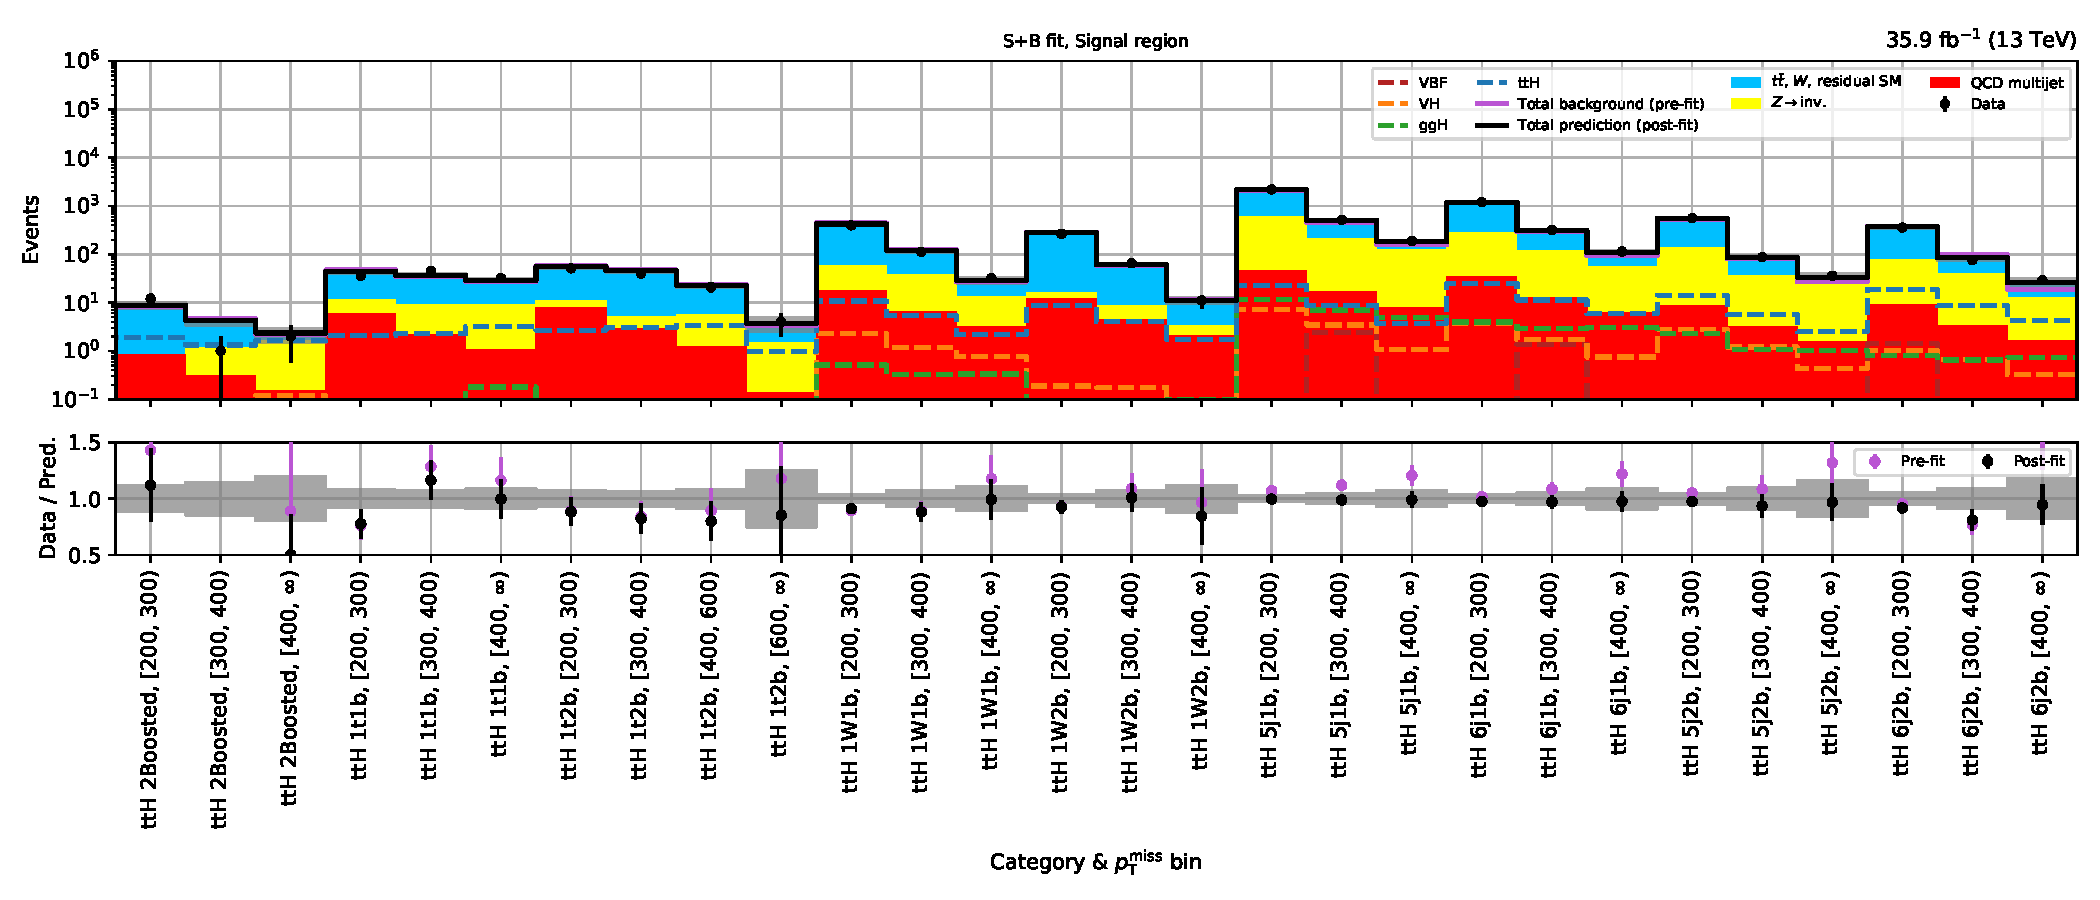
\includegraphics[width=\textwidth]{figures/mountain_ranges/2016/ttH/SR_tree_fit_s-abs_values_ttH_cats.pdf}
        \caption{\ttH --- 2016}
    \end{subfigure}

    \begin{subfigure}[b]{0.9\textwidth}
        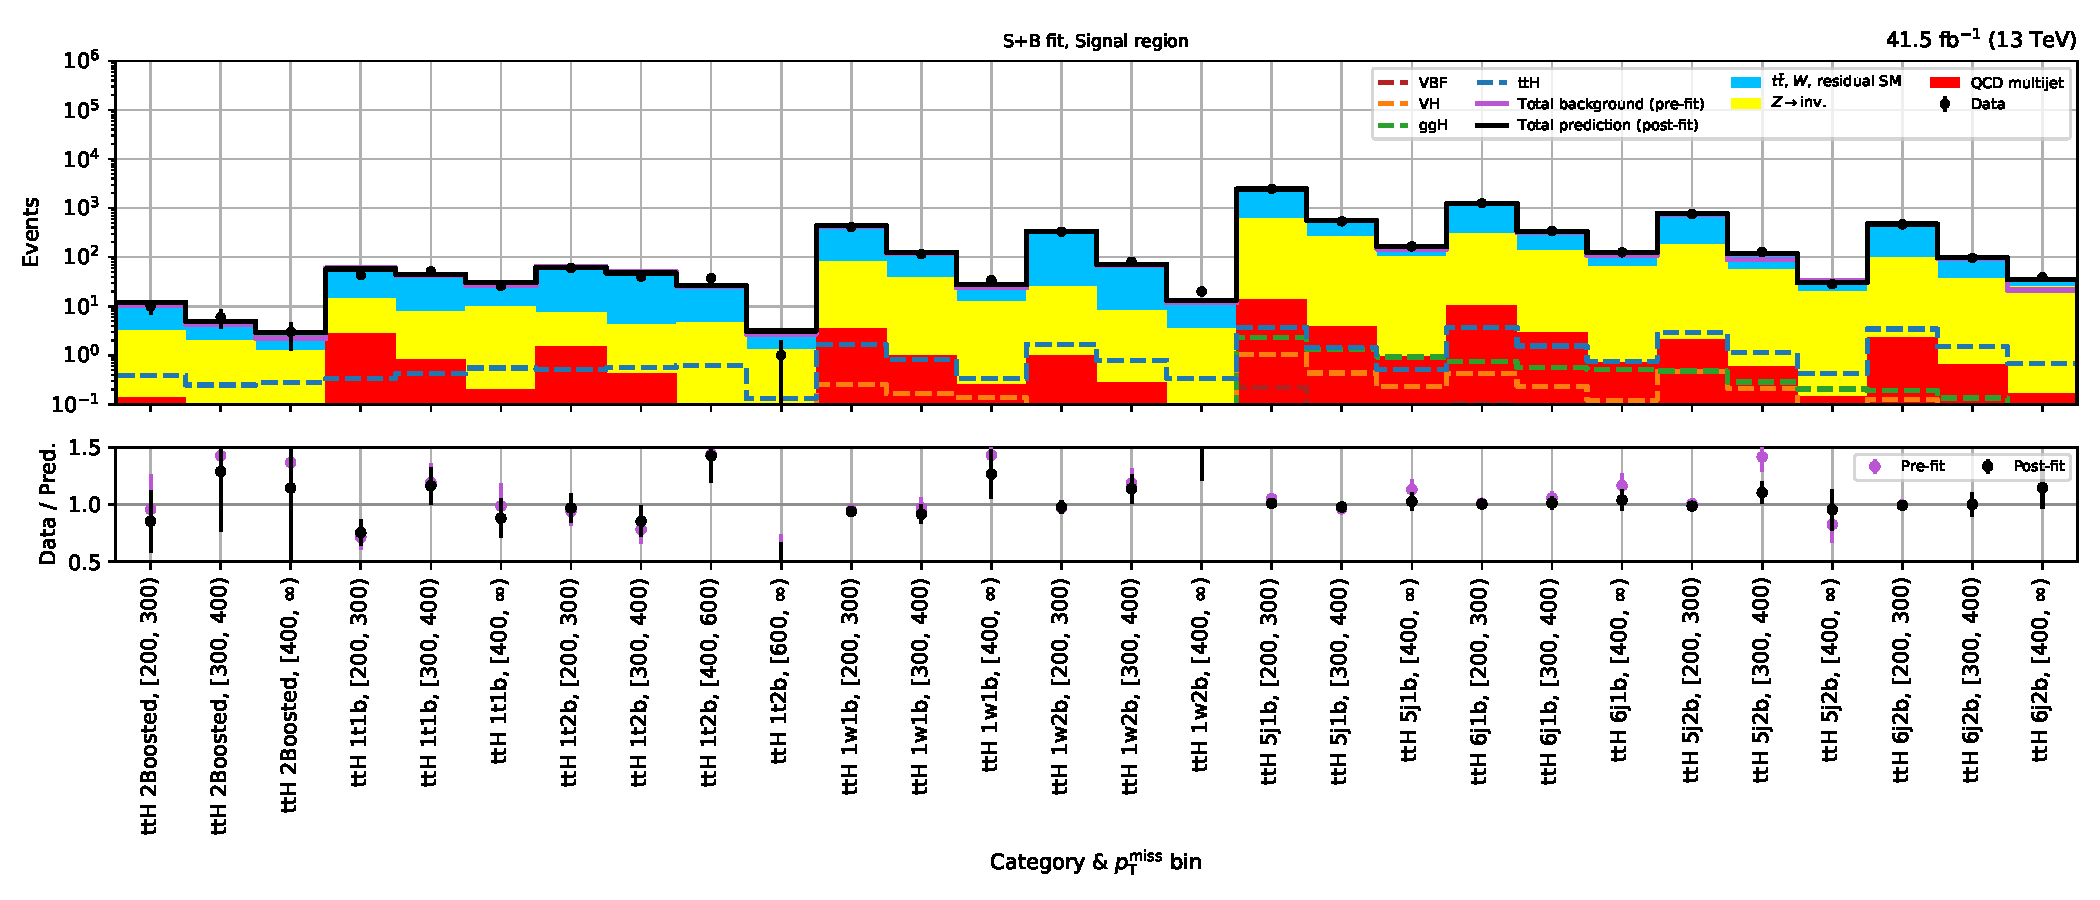
\includegraphics[width=\textwidth]{figures/mountain_ranges/2017/ttH/SR_tree_fit_s-abs_values_ttH_cats.pdf}
        \caption{\ttH --- 2017}
    \end{subfigure}

    \begin{subfigure}[b]{0.9\textwidth}
        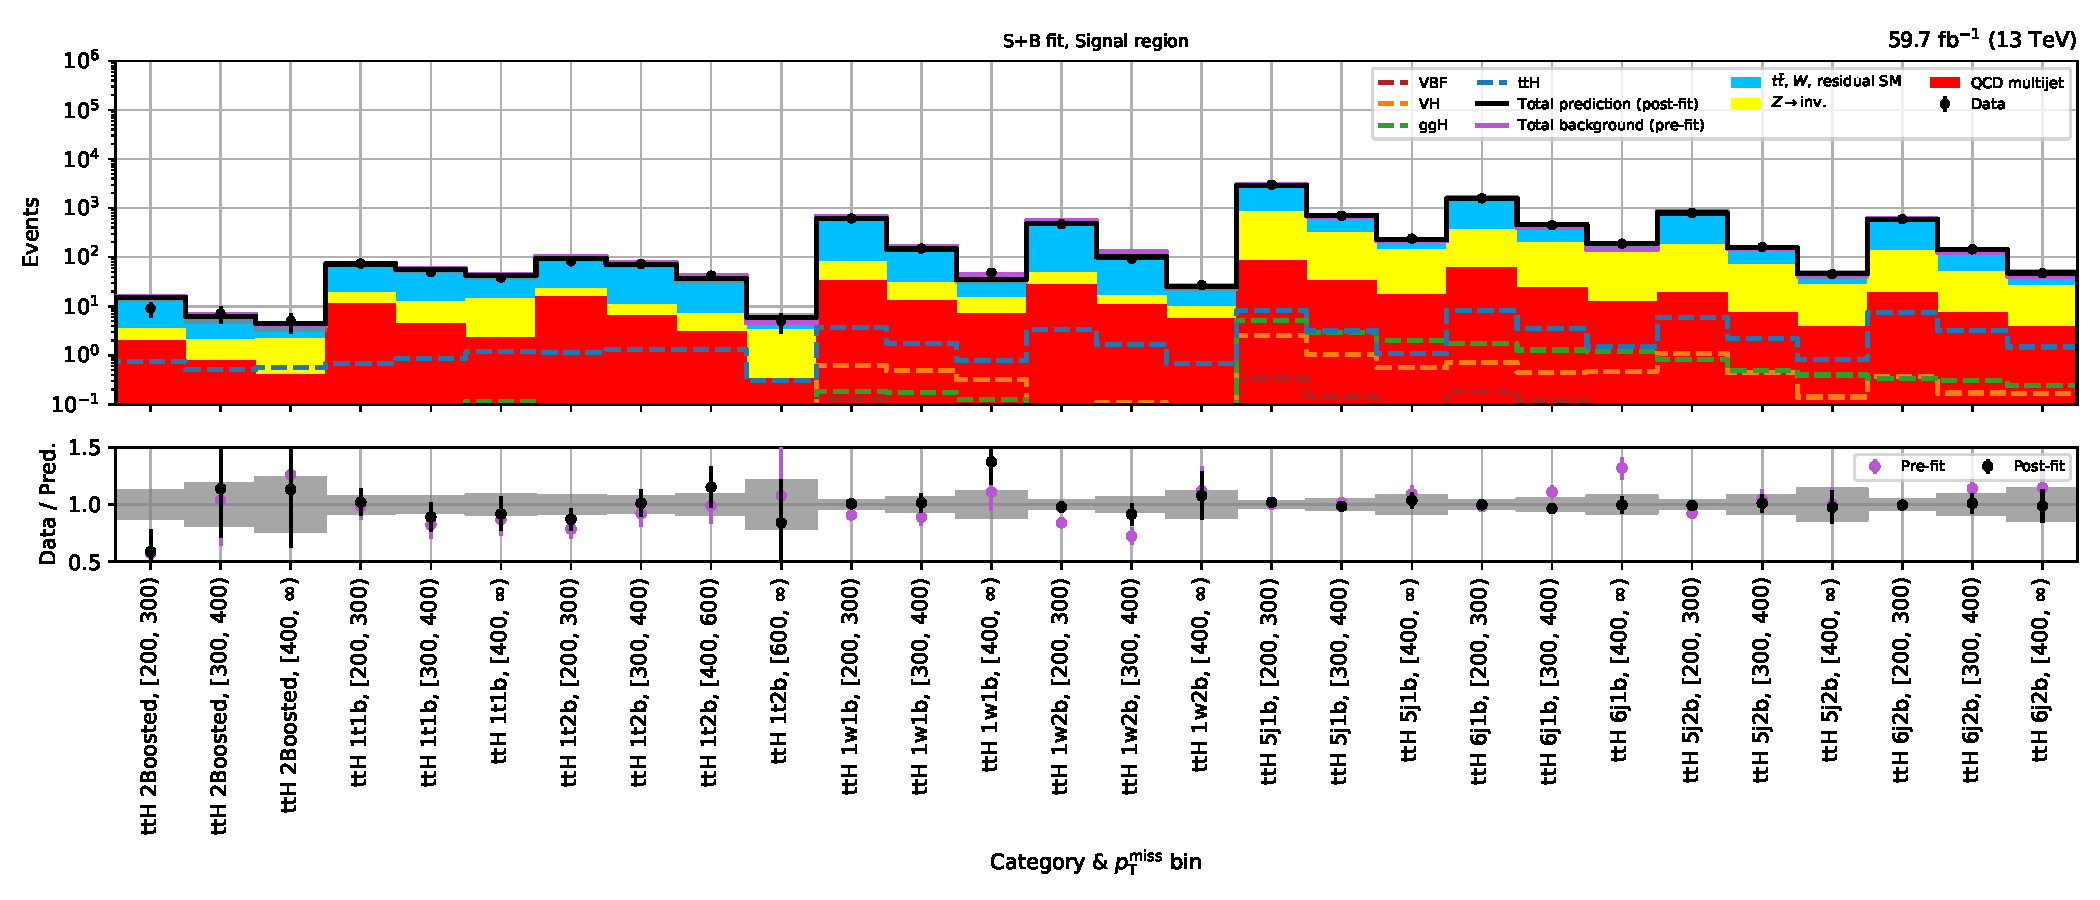
\includegraphics[width=\textwidth]{figures/mountain_ranges/2018/ttH/SR_tree_fit_s-abs_values_ttH_cats.pdf}
        \caption{\ttH --- 2018}
    \end{subfigure}
    \caption[Pre-fit and post-fit yields in the signal region for each \ttH subcategory and \ptmiss bin in each year of Run-2]{Pre-fit and post-fit yields in the signal region for each \ttH subcategory and \ptmiss bin in each year of Run-2.}
    \label{fig:htoinv_mountain_range_ttH_SR}
\end{figure}

Results of the fit tot data are presented in terms of the upper limit on the signal strength parameter \BRHinvFull. The observed limit in the signal plus background hypothesis at 95\,\% confidence level is overlaid on the expectation from the background-only hypothesis. In the latter, the median expected limit is illustrated with accompanying boundaries for the 68\,\% and 95\,\% confidence level intervals. Fig.~\ref{fig:htoinv_limit_ttH} showcases the limit and profile likelihood scan for the \ttH category in each data taking year individually and the combination over the full Run-2 dataset. Limits broken down by subcategory in each year are presented in Fig.~\ref{fig:htoinv_limit_ttH_per_year}.\footnote{Add at least a paragraph discussing the limits, and their consistency, once I have the final results. Indicate problems and stuff. Relate limits to the mountain ranges.}

\begin{figure}[htbp]
    \centering
    \begin{subfigure}[b]{0.45\textwidth}
        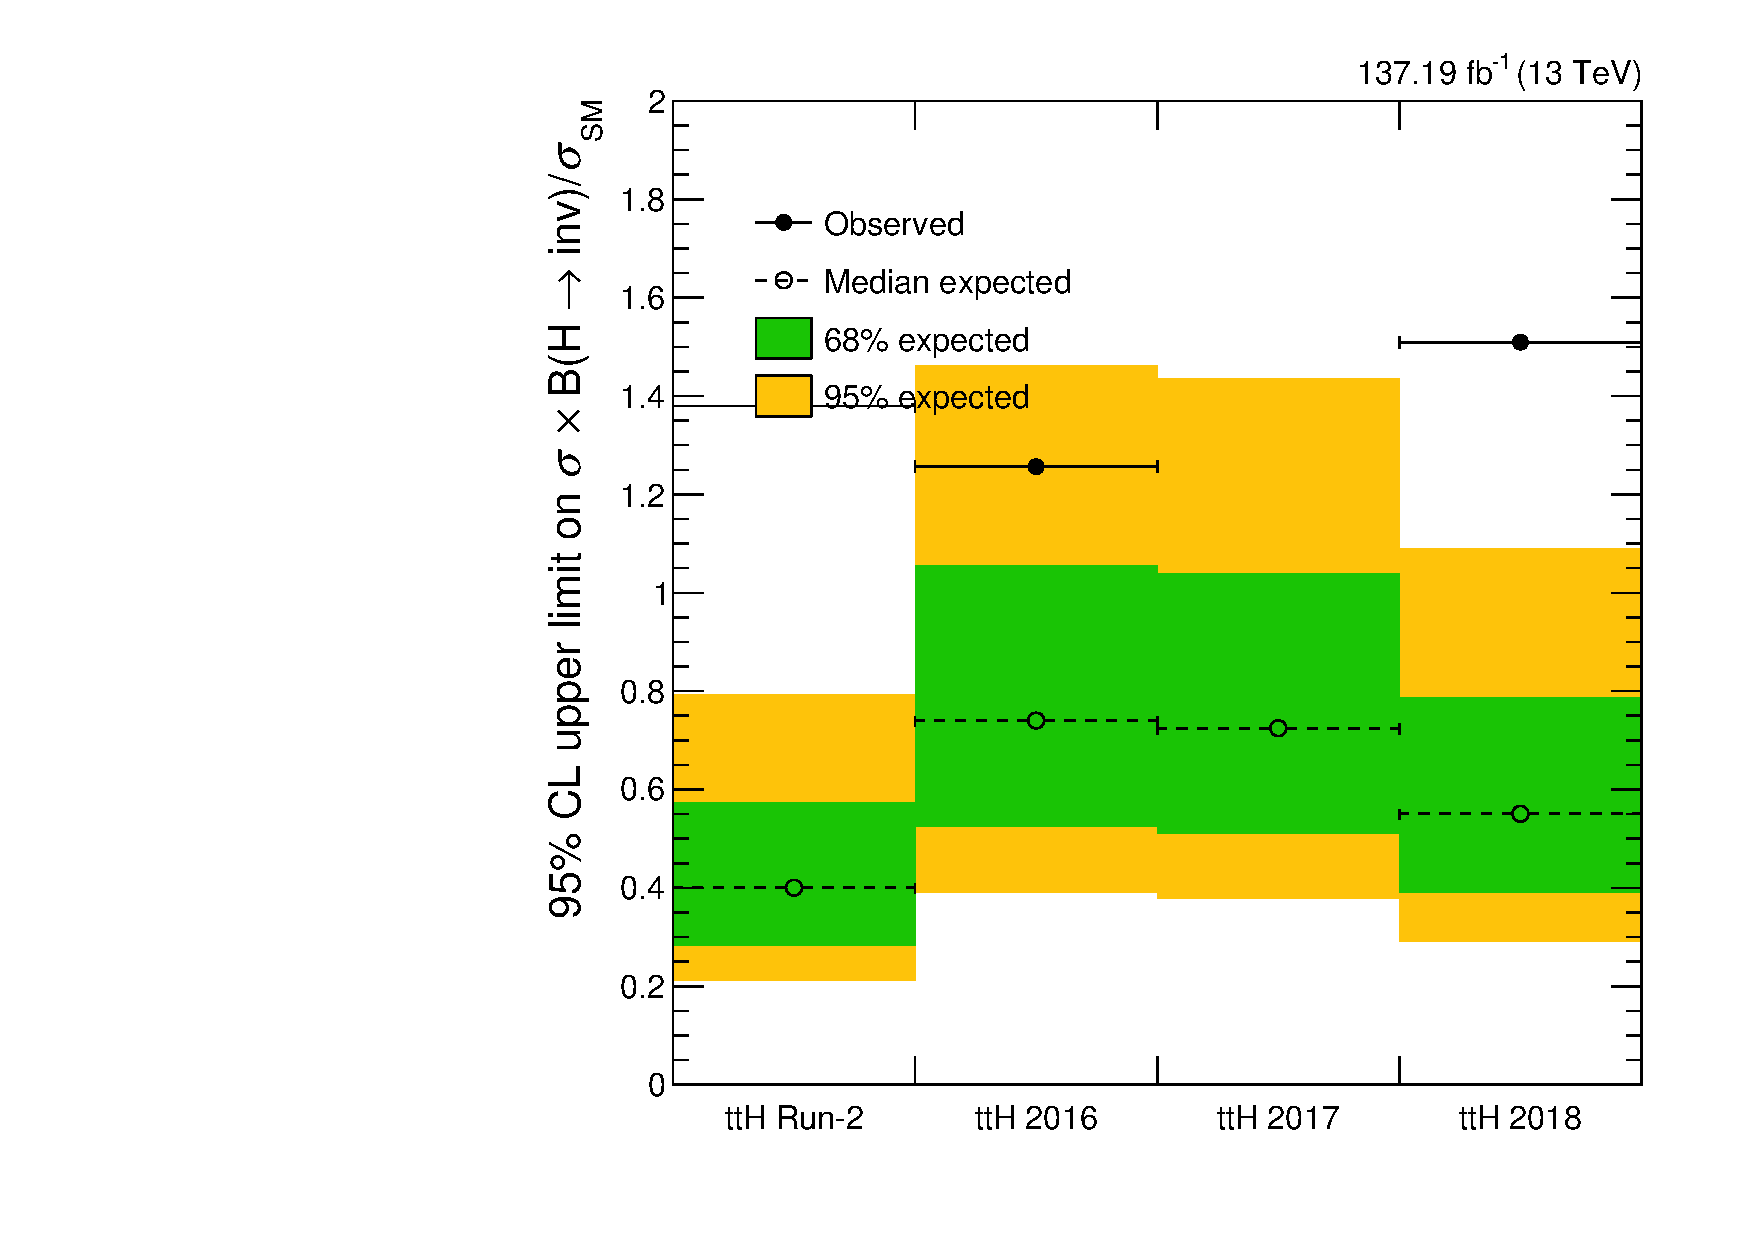
\includegraphics[width=\textwidth]{figures/limits/ttH/limit_Run2_ttH.pdf}
        \caption{Limit --- \ttH}
    \end{subfigure}
    \hspace{0.05\textwidth}
    \begin{subfigure}[t]{0.45\textwidth}
        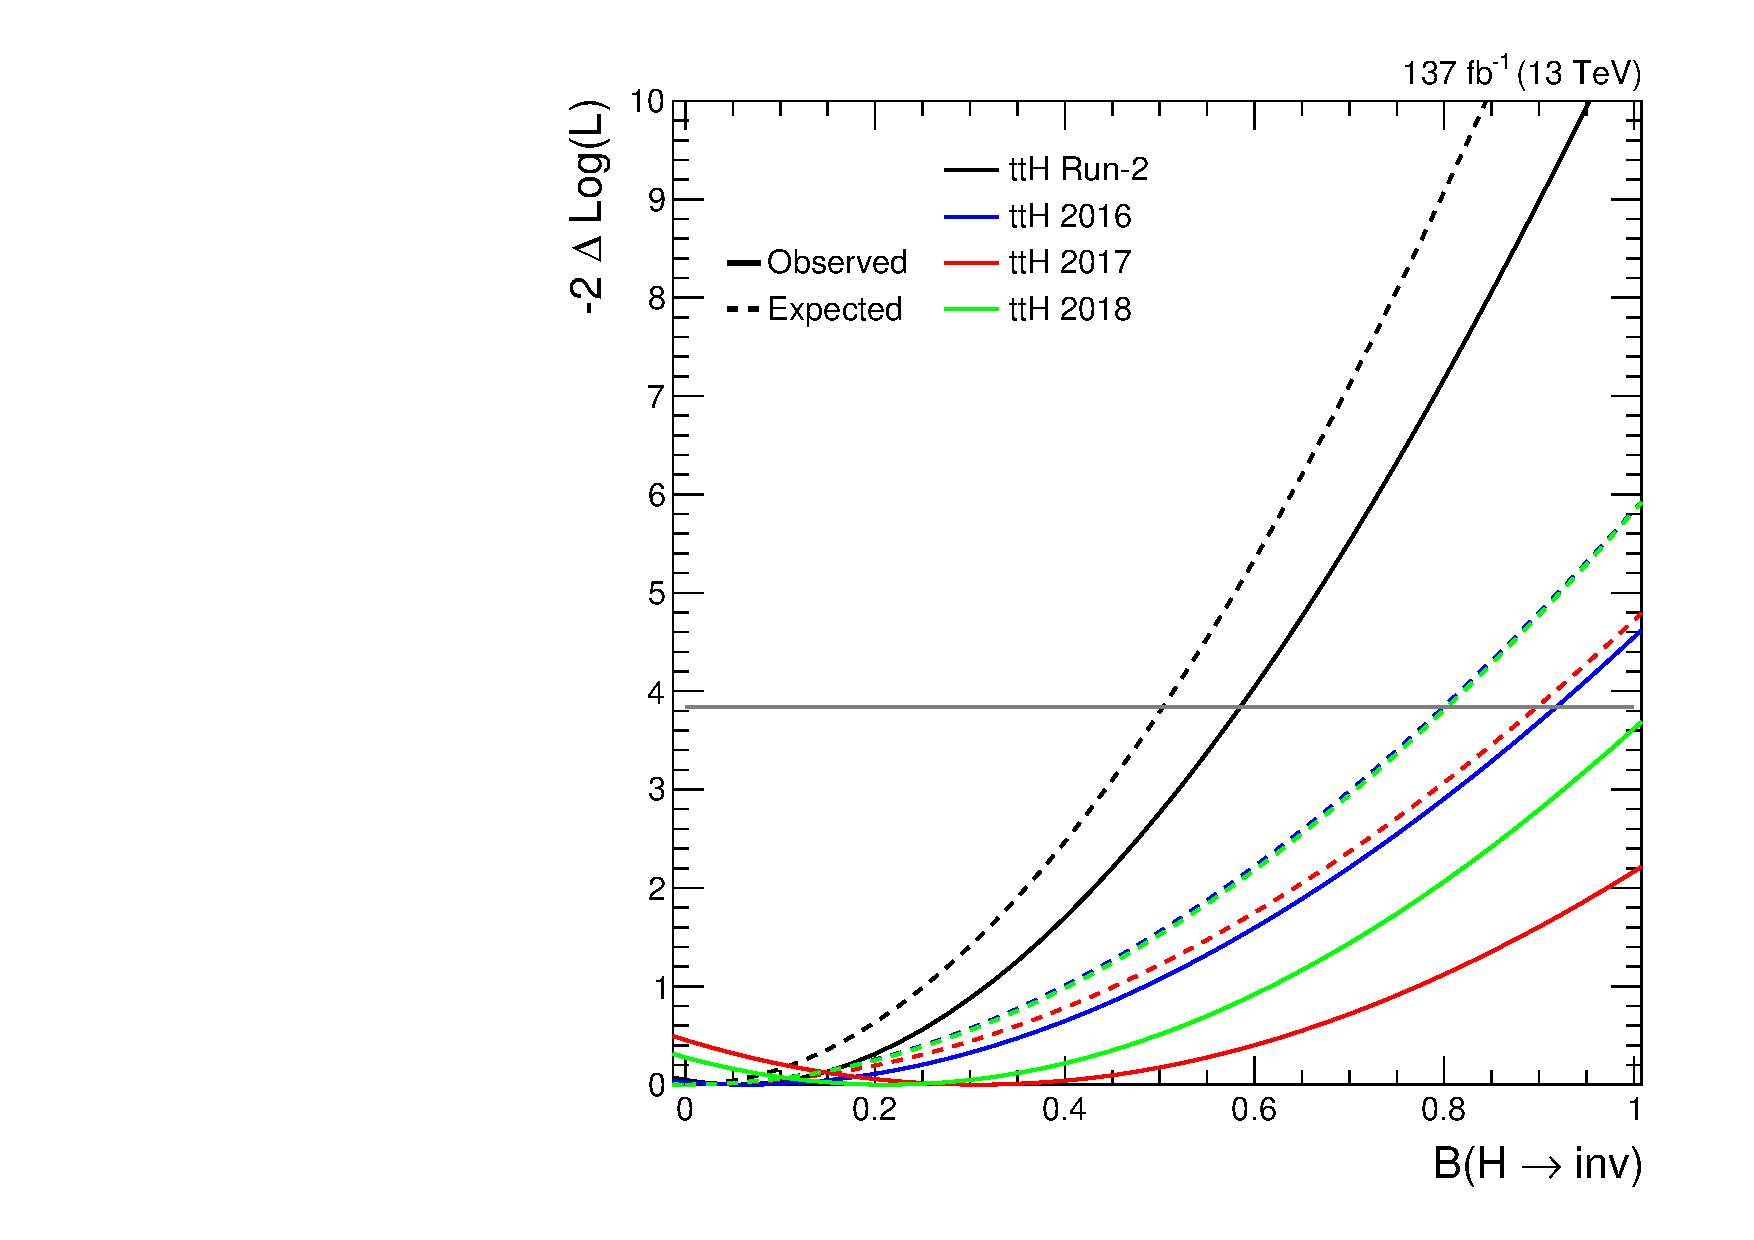
\includegraphics[width=\textwidth]{figures/likelihood_scan/profile_likelihood_scan_Run2_ttH.pdf}
        \caption{Profile likelihood --- \ttH}
    \end{subfigure}
    \caption[Observed and expected 95\,\% CL upper limit on the Higgs boson to invisible state branching fraction $\BRof{\higgstoinv}$ (left) and the corresponding profile likelihood ratio as a function of it (right) in the \ttH category]{Observed and expected 95\,\% CL upper limit on the Higgs boson to invisible state branching fraction $\BRof{\higgstoinv}$ (left) and the corresponding profile likelihood ratio as a function of it (right) in the \ttH category. The result from each data taking period is presented along with their combination.}
    \label{fig:htoinv_limit_ttH}
\end{figure}

\clearpage


%=========================================================


\subsection{Results of the \texorpdfstring{\VH}{VH} analysis}
\label{subsec:htoinv_analysis_VH}

Contrary to \ttH, all of the \glspl{CR} are utilised in the non-multijet background predictions. A more accurate \ztonunu prediction is possible since it can be constrained by three \glspl{CR}. Events with a \VH topology, being characterised by a dijet pair or single fat jet recoiling from the \ptvecmiss, naturally has a large \mindphi. Predicting the \acrshort{qcd} multijet background in the signal region using the any of the sidebands inverted in this variable was therefore not possible. The sidebands inverted in \omegaTilde contained little \acrshort{qcd} to extrapolate from. Therefore, the tight double sideband from the \ggH 2jM category was chosen as it, too, has a dijet topology, but an inverted dijet mass requirement that populates it sufficiently with multijet events.

Distributions of the pre-fit and post-fit yields for 2016, 2017, and 2018 are displayed in Fig.~\ref{fig:htoinv_mountain_range_VH_SR}. Corresponding figures for the \glspl{CR} are given in App.~\ref{sec:pre_post_fit_plots_VH_CRs}.\footnote{Add at least a paragraph discussing the pre-fit vs post-fit yields, i.e., how well the fit is able to model the background/allow it to fill any pre-fit data excesses, once I have the final results.}

\begin{figure}[htbp]
    \centering
    \begin{subfigure}[b]{0.9\textwidth}
        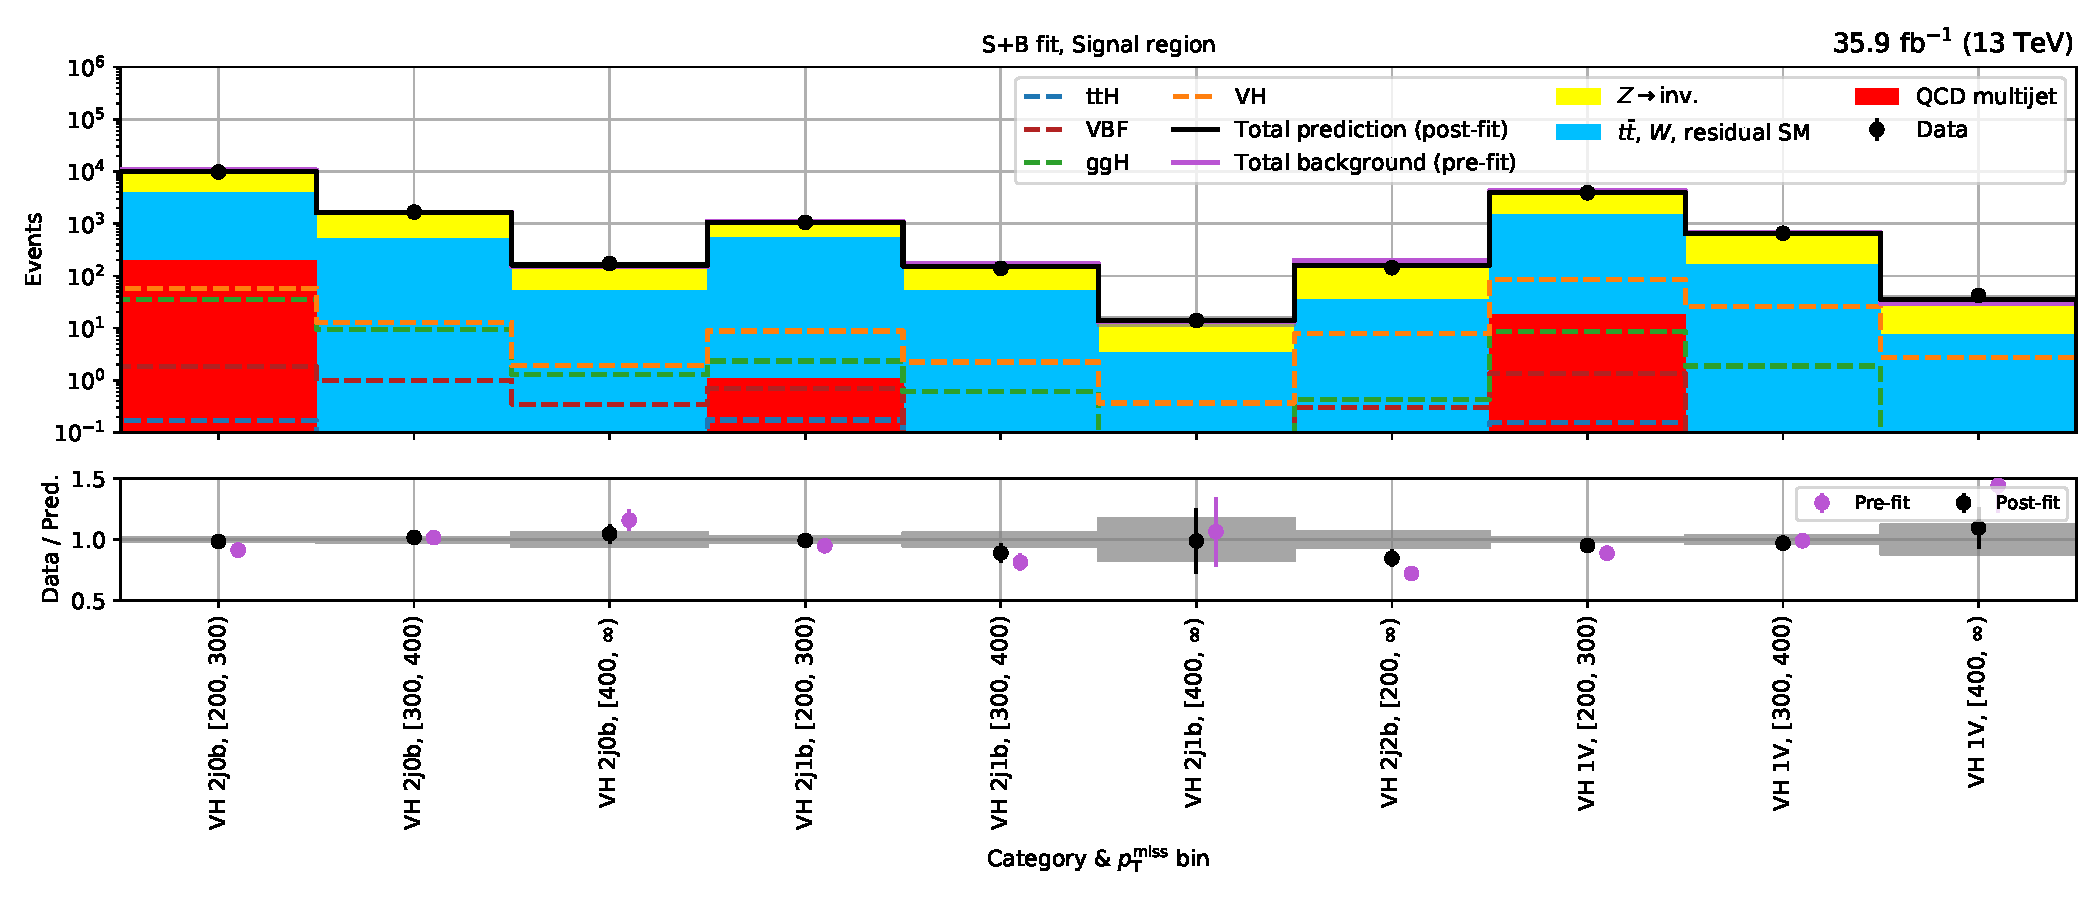
\includegraphics[width=\textwidth]{figures/mountain_ranges/2016/VH/SR_tree_fit_s-abs_values_VH_cats.pdf}
        \caption{\VH --- 2016}
    \end{subfigure}

    \begin{subfigure}[b]{0.9\textwidth}
        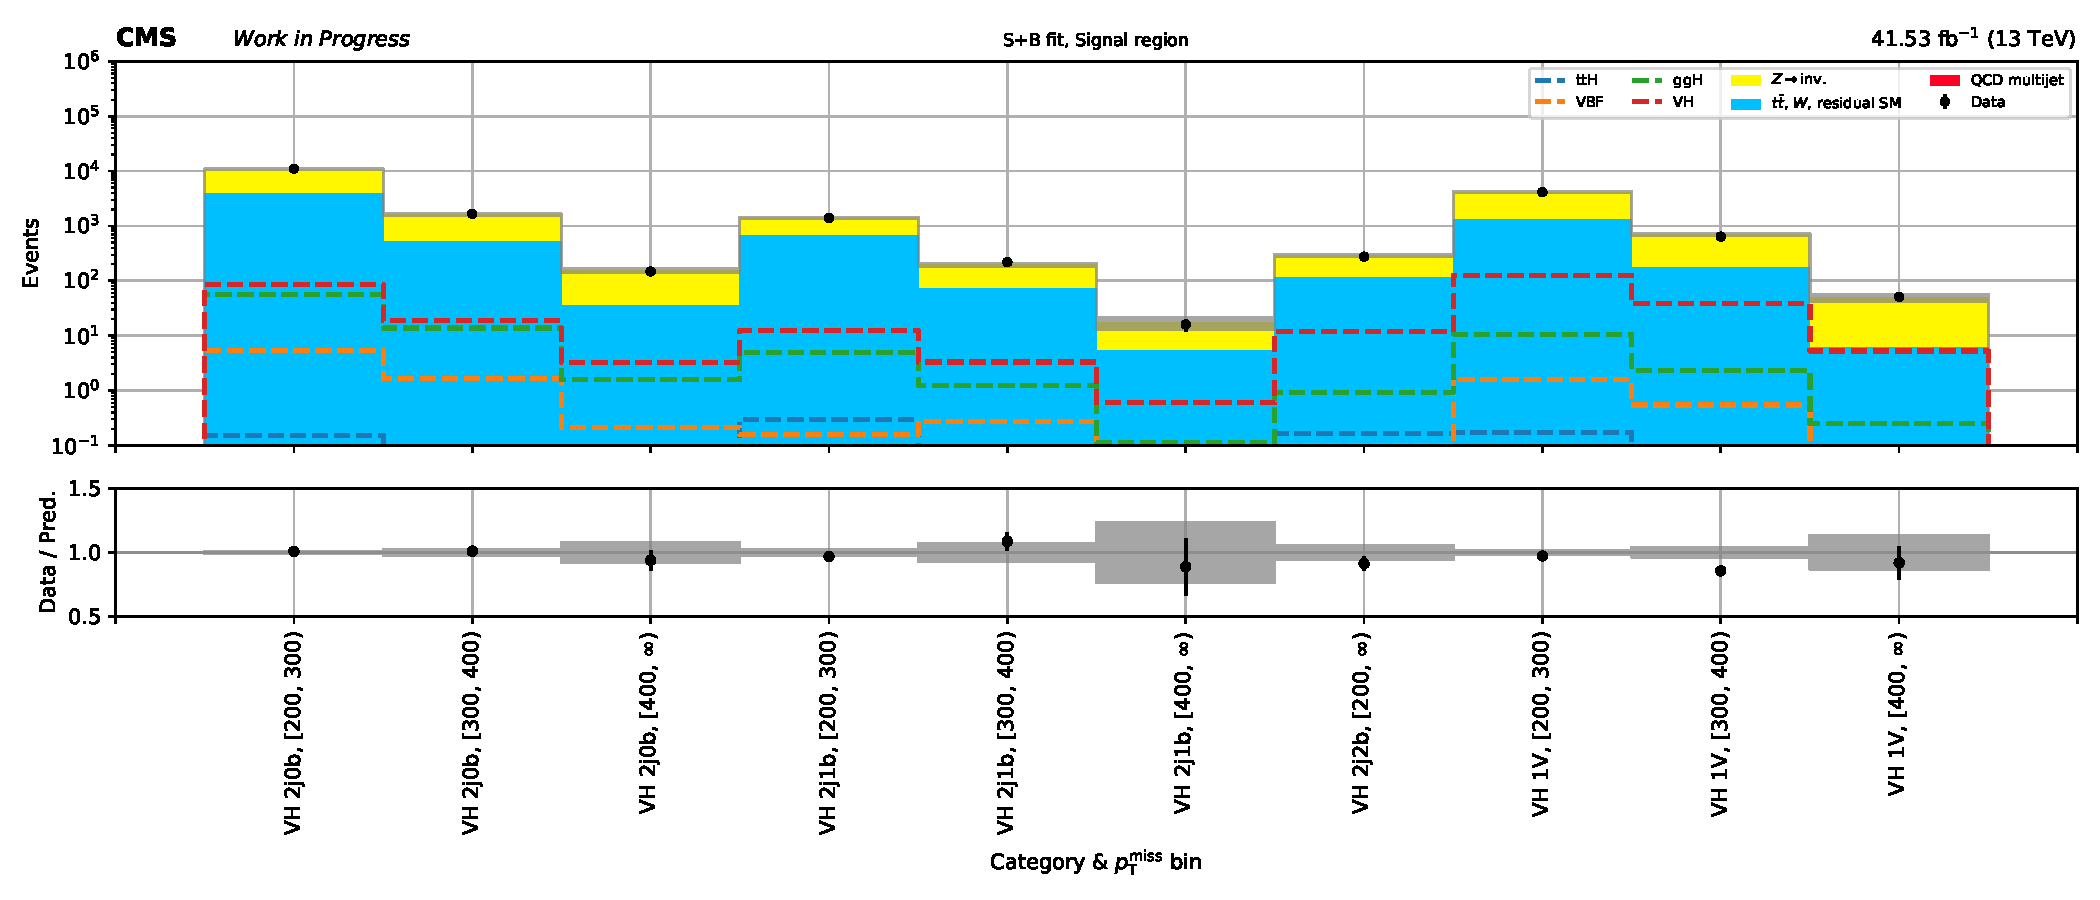
\includegraphics[width=\textwidth]{figures/mountain_ranges/2017/VH/SR_tree_fit_s-abs_values_VH_cats.pdf}
        \caption{\VH --- 2017}
    \end{subfigure}

    \begin{subfigure}[b]{0.9\textwidth}
        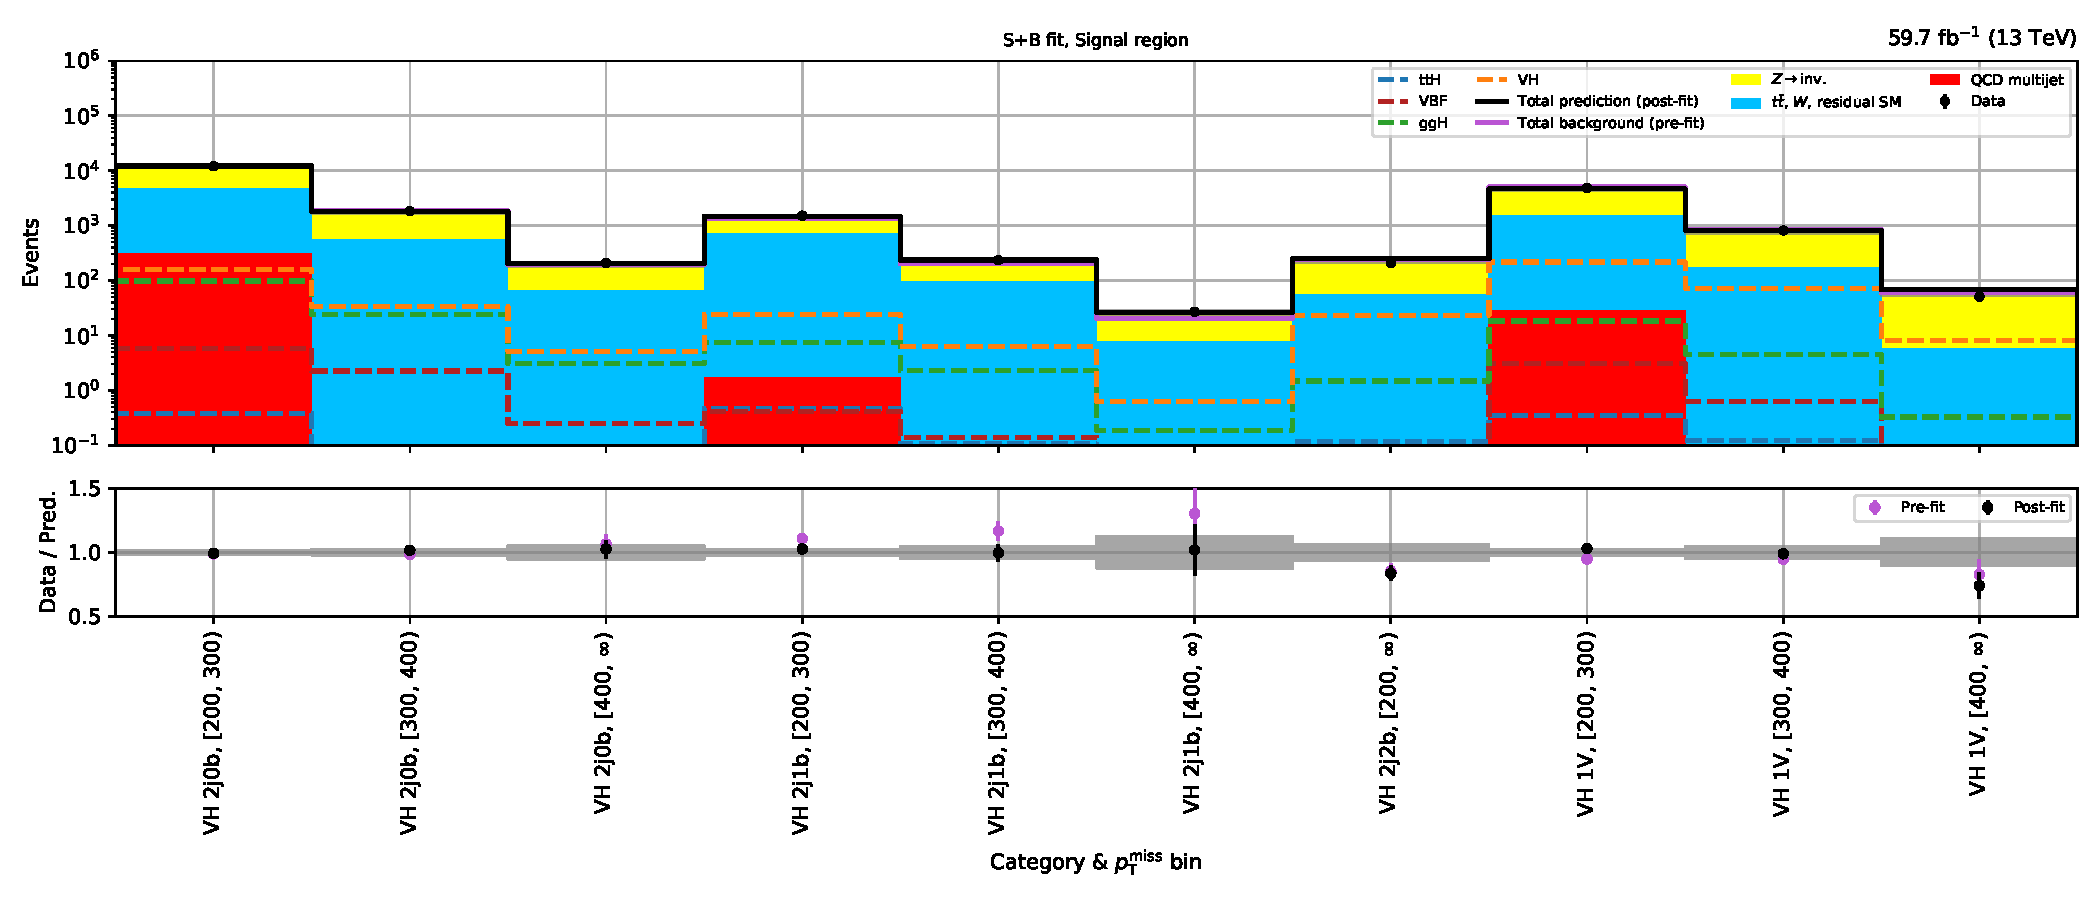
\includegraphics[width=\textwidth]{figures/mountain_ranges/2018/VH/SR_tree_fit_s-abs_values_VH_cats.pdf}
        \caption{\VH --- 2018}
    \end{subfigure}
    \caption[Pre-fit and post-fit yields in the signal region for each \VH subcategory and \ptmiss bin in each year of Run-2]{Pre-fit and post-fit yields in the signal region for each \VH subcategory and \ptmiss bin in each year of Run-2.}
    \label{fig:htoinv_mountain_range_VH_SR}
\end{figure}

Fig.~\ref{fig:htoinv_limit_VH} showcases the expected and observed limits for the \VH category in each year and the Run-2 combination. Limits for each subcategory can be found in Fig.~\ref{fig:htoinv_limit_VH_per_year}.\footnote{Add at least a paragraph discussing the limits, and their consistency, once I have the final results. Indicate problems and stuff. Relate limits to the mountain ranges.}

\begin{figure}[htbp]
    \centering
    \begin{subfigure}[b]{0.45\textwidth}
        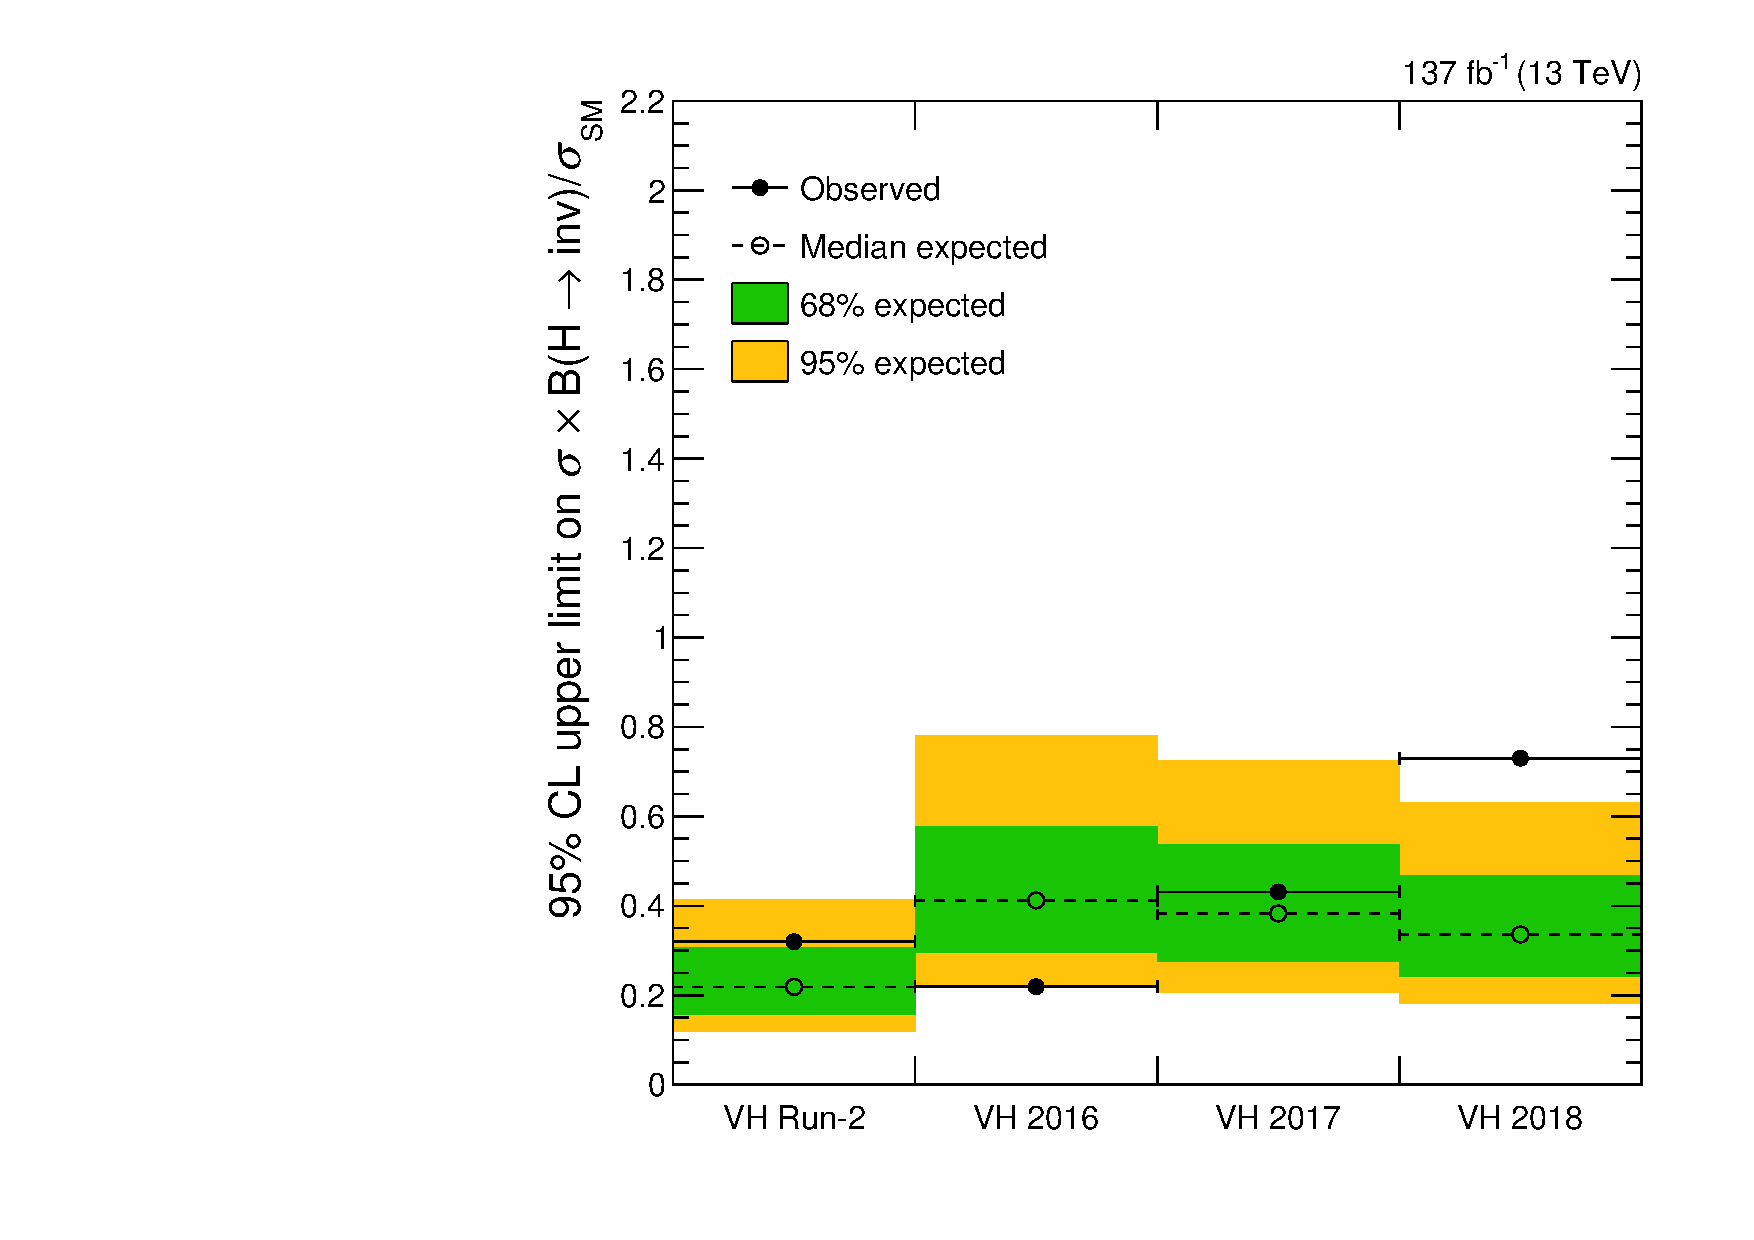
\includegraphics[width=\textwidth]{figures/limits/VH/limit_Run2_VH.pdf}
        \caption{Limit --- \VH}
    \end{subfigure}
    \hspace{0.05\textwidth}
    \begin{subfigure}[t]{0.45\textwidth}
        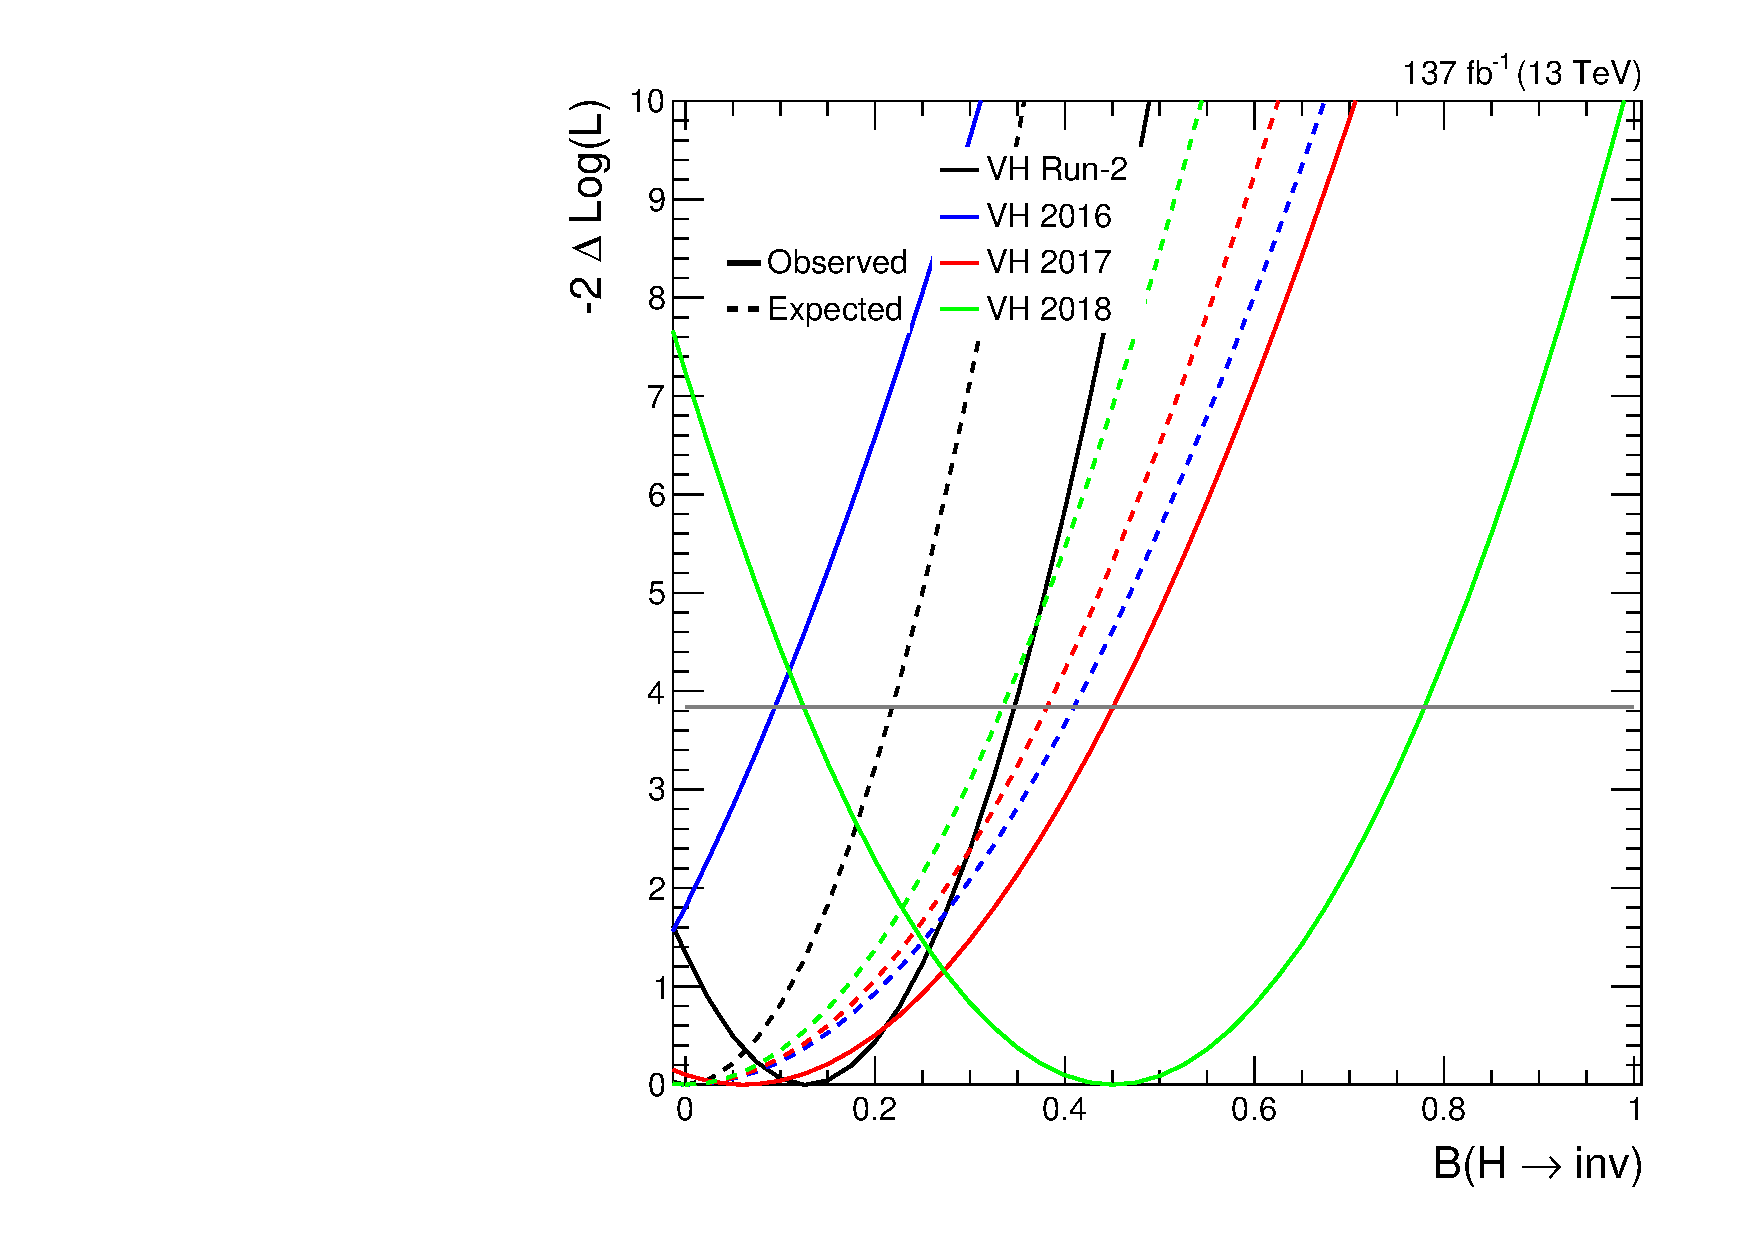
\includegraphics[width=\textwidth]{figures/likelihood_scan/profile_likelihood_scan_Run2_VH.pdf}
        \caption{Profile likelihood --- \VH}
    \end{subfigure}
    \caption[Observed and expected 95\,\% CL upper limit on the Higgs boson to invisible state branching fraction $\BRof{\higgstoinv}$ (left) and the corresponding profile likelihood ratio as a function of it (right) in the \VH category]{Observed and expected 95\,\% CL upper limit on the Higgs boson to invisible state branching fraction $\BRof{\higgstoinv}$ (left) and the corresponding profile likelihood ratio as a function of it (right) in the \VH category. The result from each data taking period is presented along with their combination.}
    \label{fig:htoinv_limit_VH}
\end{figure}

\clearpage


%=========================================================


\subsection{Results of the \texorpdfstring{\ggH}{ggH} analysis}
\label{subsec:htoinv_analysis_ggF}

As with the \VH category, all of the \glspl{CR} are involved in estimating the non-multijet backgrounds in the signal region of the \ggH category. Equivalently to \ttH, the \acrshort{qcd} presence is derived using the \acrshort{qcd} event counts in the signal region and tight double sideband, taking advantage of the smeared multijet sample.

Distributions of the pre-fit and post-fit yields for 2016, 2017, and 2018 are displayed in Fig.~\ref{fig:htoinv_mountain_range_ggH_SR}. Corresponding figures for the \glspl{CR} are given in App.~\ref{sec:pre_post_fit_plots_ggF_CRs}.\footnote{Add at least a paragraph discussing the pre-fit vs post-fit yields, i.e., how well the fit is able to model the background/allow it to fill any pre-fit data excesses, once I have the final results.}

\begin{figure}[htbp]
    \centering
    \begin{subfigure}[b]{0.9\textwidth}
        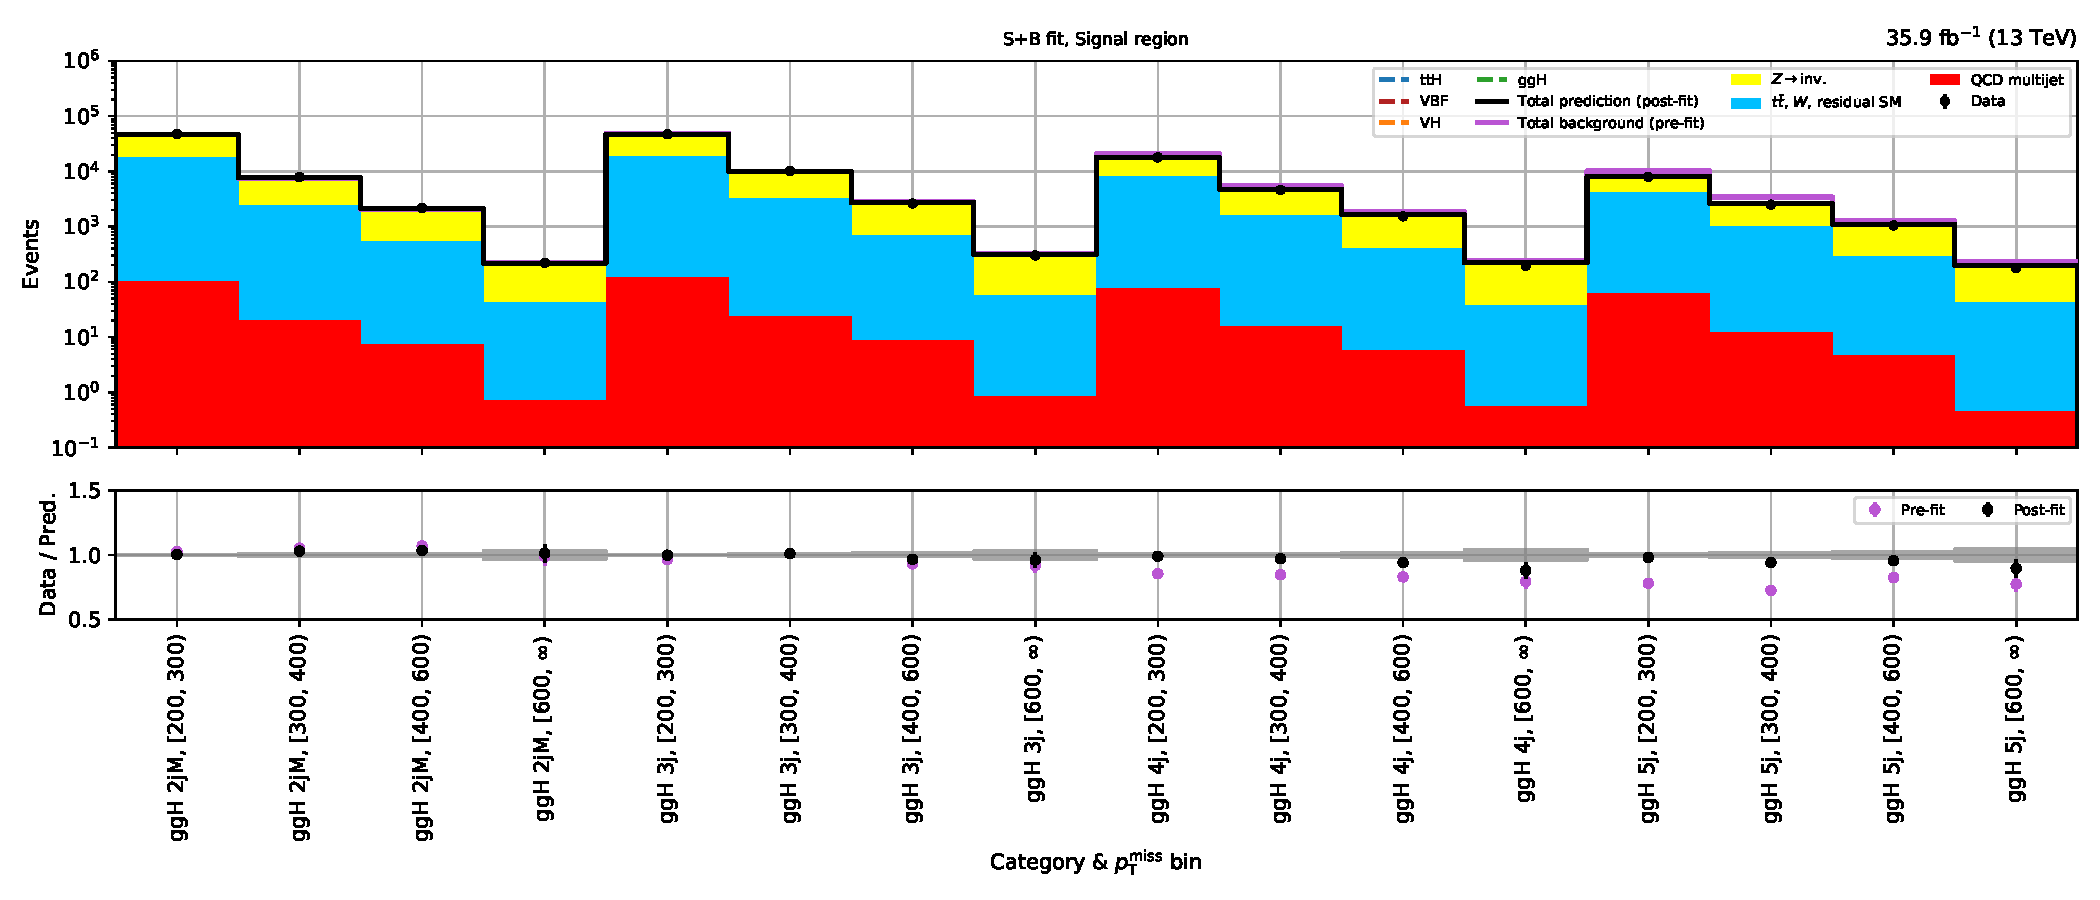
\includegraphics[width=\textwidth]{figures/mountain_ranges/2016/ggF/SR_tree_fit_s-abs_values_ggF_cats.pdf}
        \caption{\ggH --- 2016}
    \end{subfigure}

    \begin{subfigure}[b]{0.9\textwidth}
        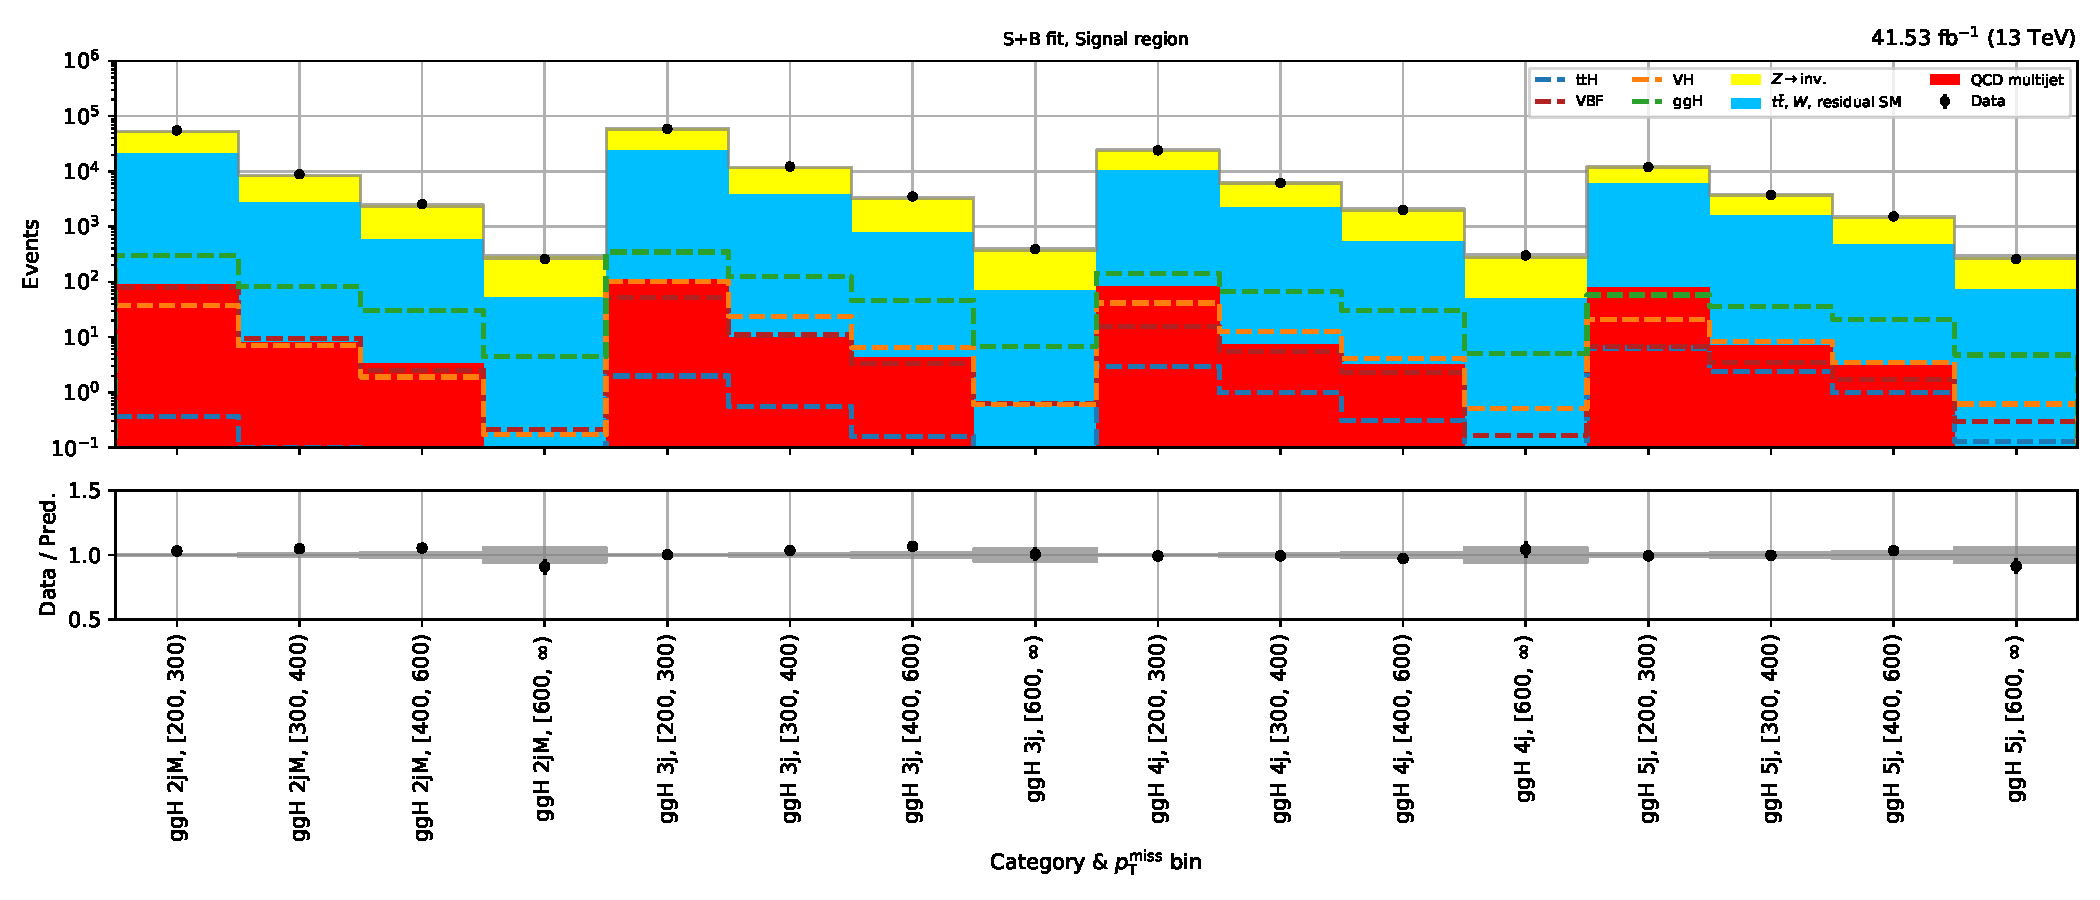
\includegraphics[width=\textwidth]{figures/mountain_ranges/2017/ggF/SR_tree_fit_s-abs_values_ggF_cats.pdf}
        \caption{\ggH --- 2017}
    \end{subfigure}

    \begin{subfigure}[b]{0.9\textwidth}
        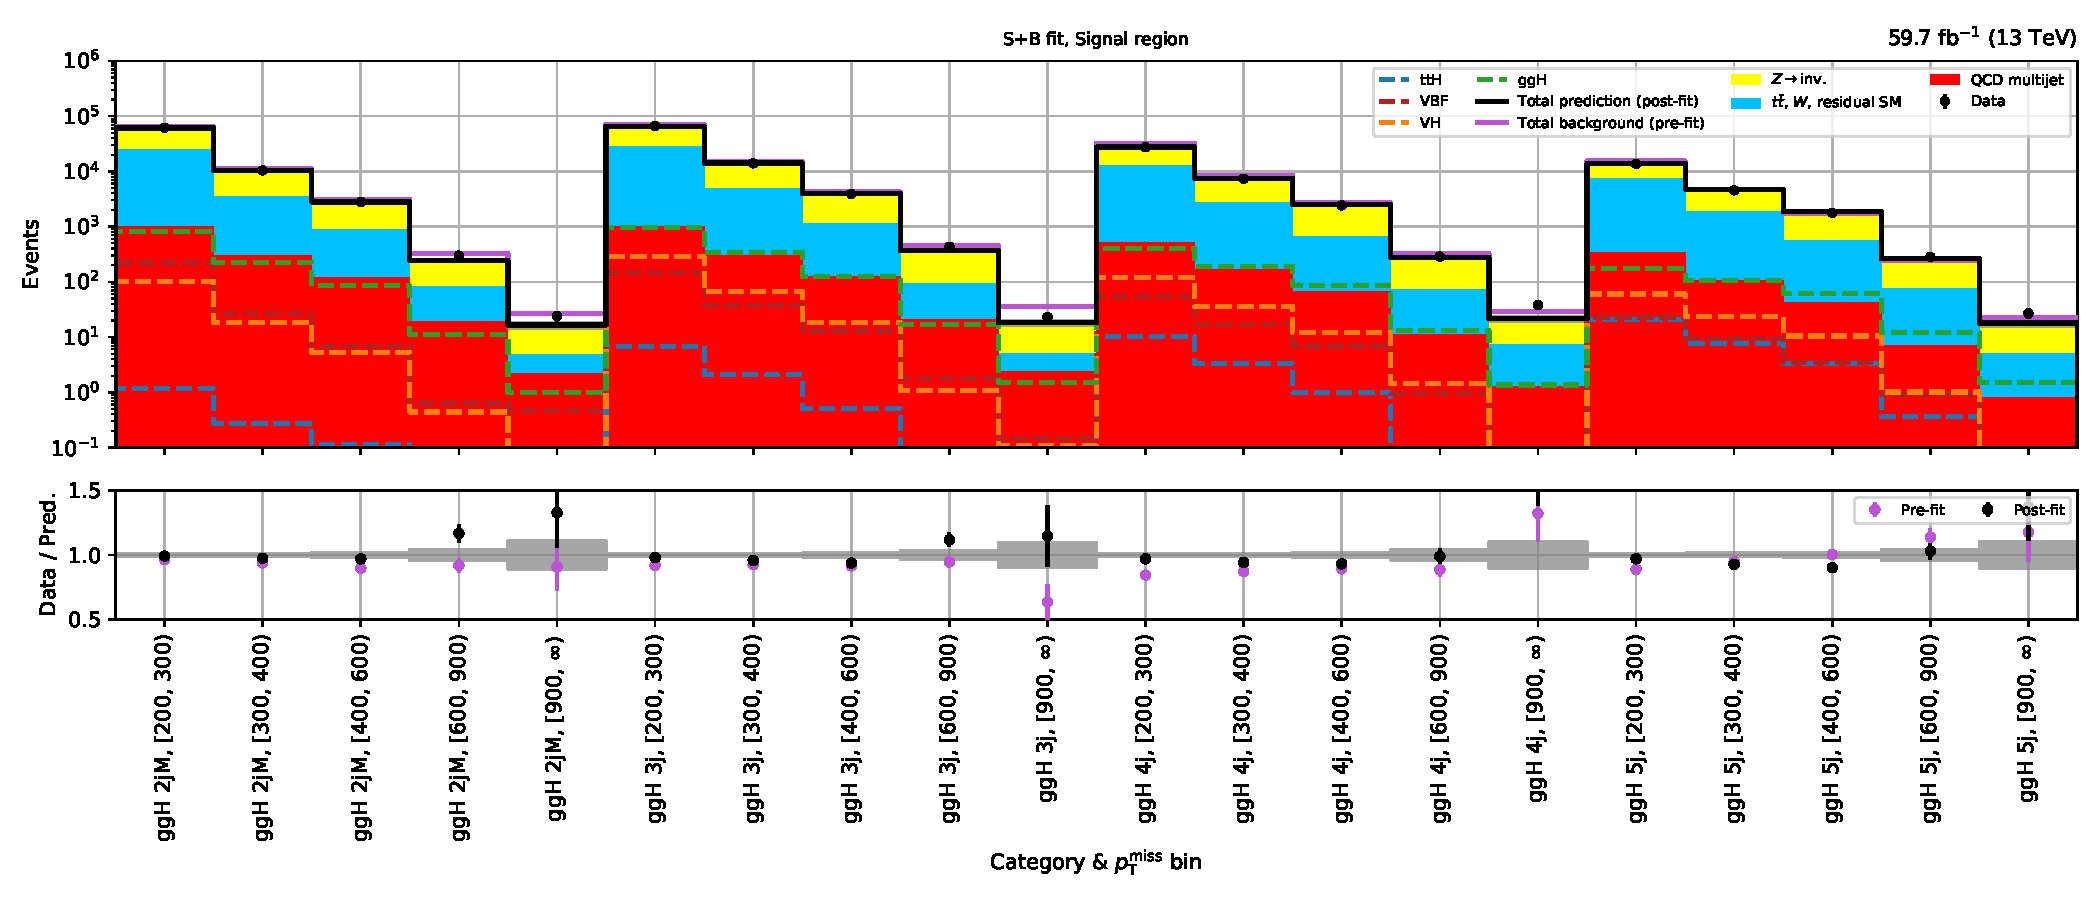
\includegraphics[width=\textwidth]{figures/mountain_ranges/2018/ggF/SR_tree_fit_s-abs_values_ggF_cats.pdf}
        \caption{\ggH --- 2018}
    \end{subfigure}
    \caption[Pre-fit and post-fit yields in the signal region for each \ggH subcategory and \ptmiss bin in each year of Run-2]{Pre-fit and post-fit yields in the signal region for each \ggH subcategory and \ptmiss bin in each year of Run-2.}
    \label{fig:htoinv_mountain_range_ggH_SR}
\end{figure}

Expected and observed limits on the signal strength parameter are presented in Fig.~\ref{fig:htoinv_limit_ggF} for the \ggH category for the full Run-2 dataset as well as broken down by year. A further breakdown by category is given in Fig.~\ref{fig:htoinv_limit_ggH_per_year}.\footnote{Add at least a paragraph discussing the limits, and their consistency, once I have the final results. Indicate problems and stuff. Relate limits to the mountain ranges.}

\begin{figure}[htbp]
    \centering
    \begin{subfigure}[b]{0.45\textwidth}
        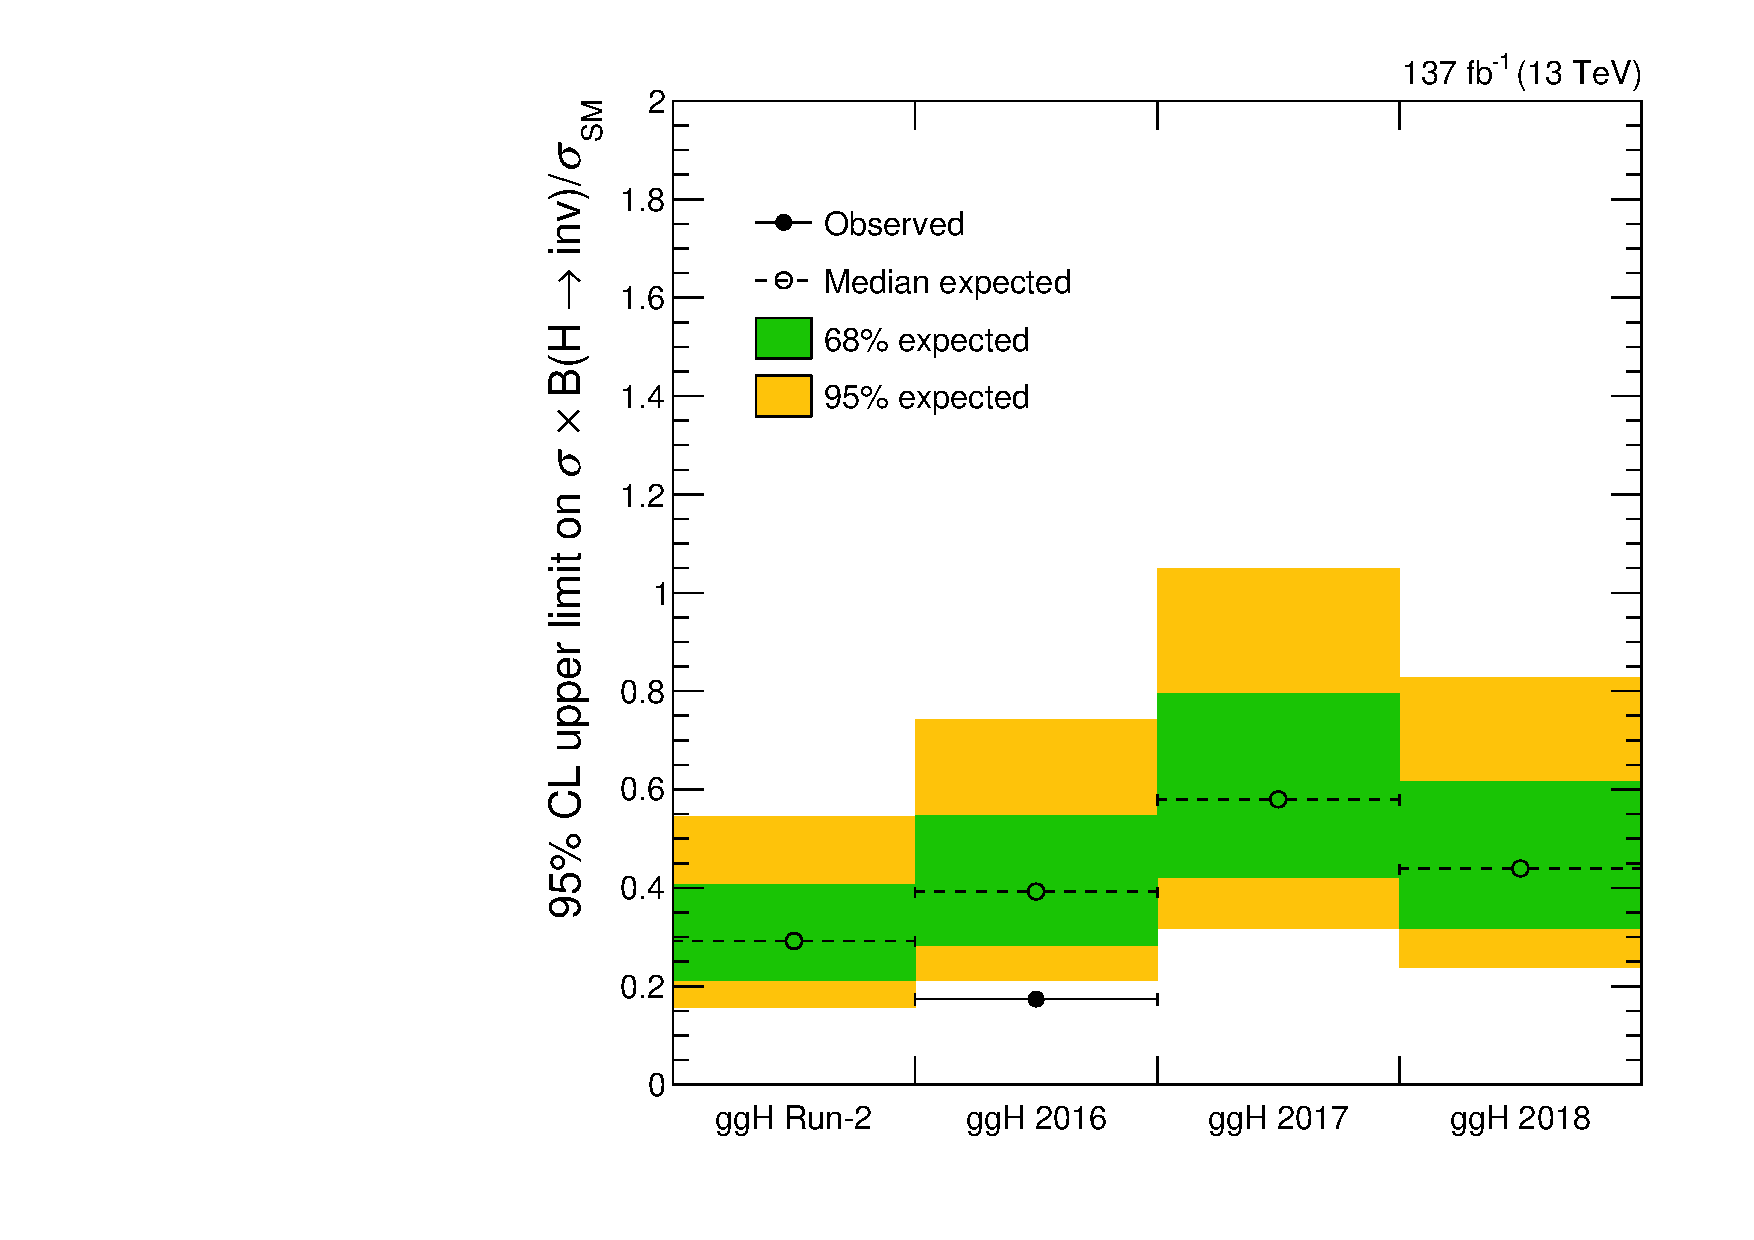
\includegraphics[width=\textwidth]{figures/limits/ggF/limit_Run2_ggF.pdf}
        \caption{Limit --- \ggH}
    \end{subfigure}
    \hspace{0.05\textwidth}
    \begin{subfigure}[t]{0.45\textwidth}
        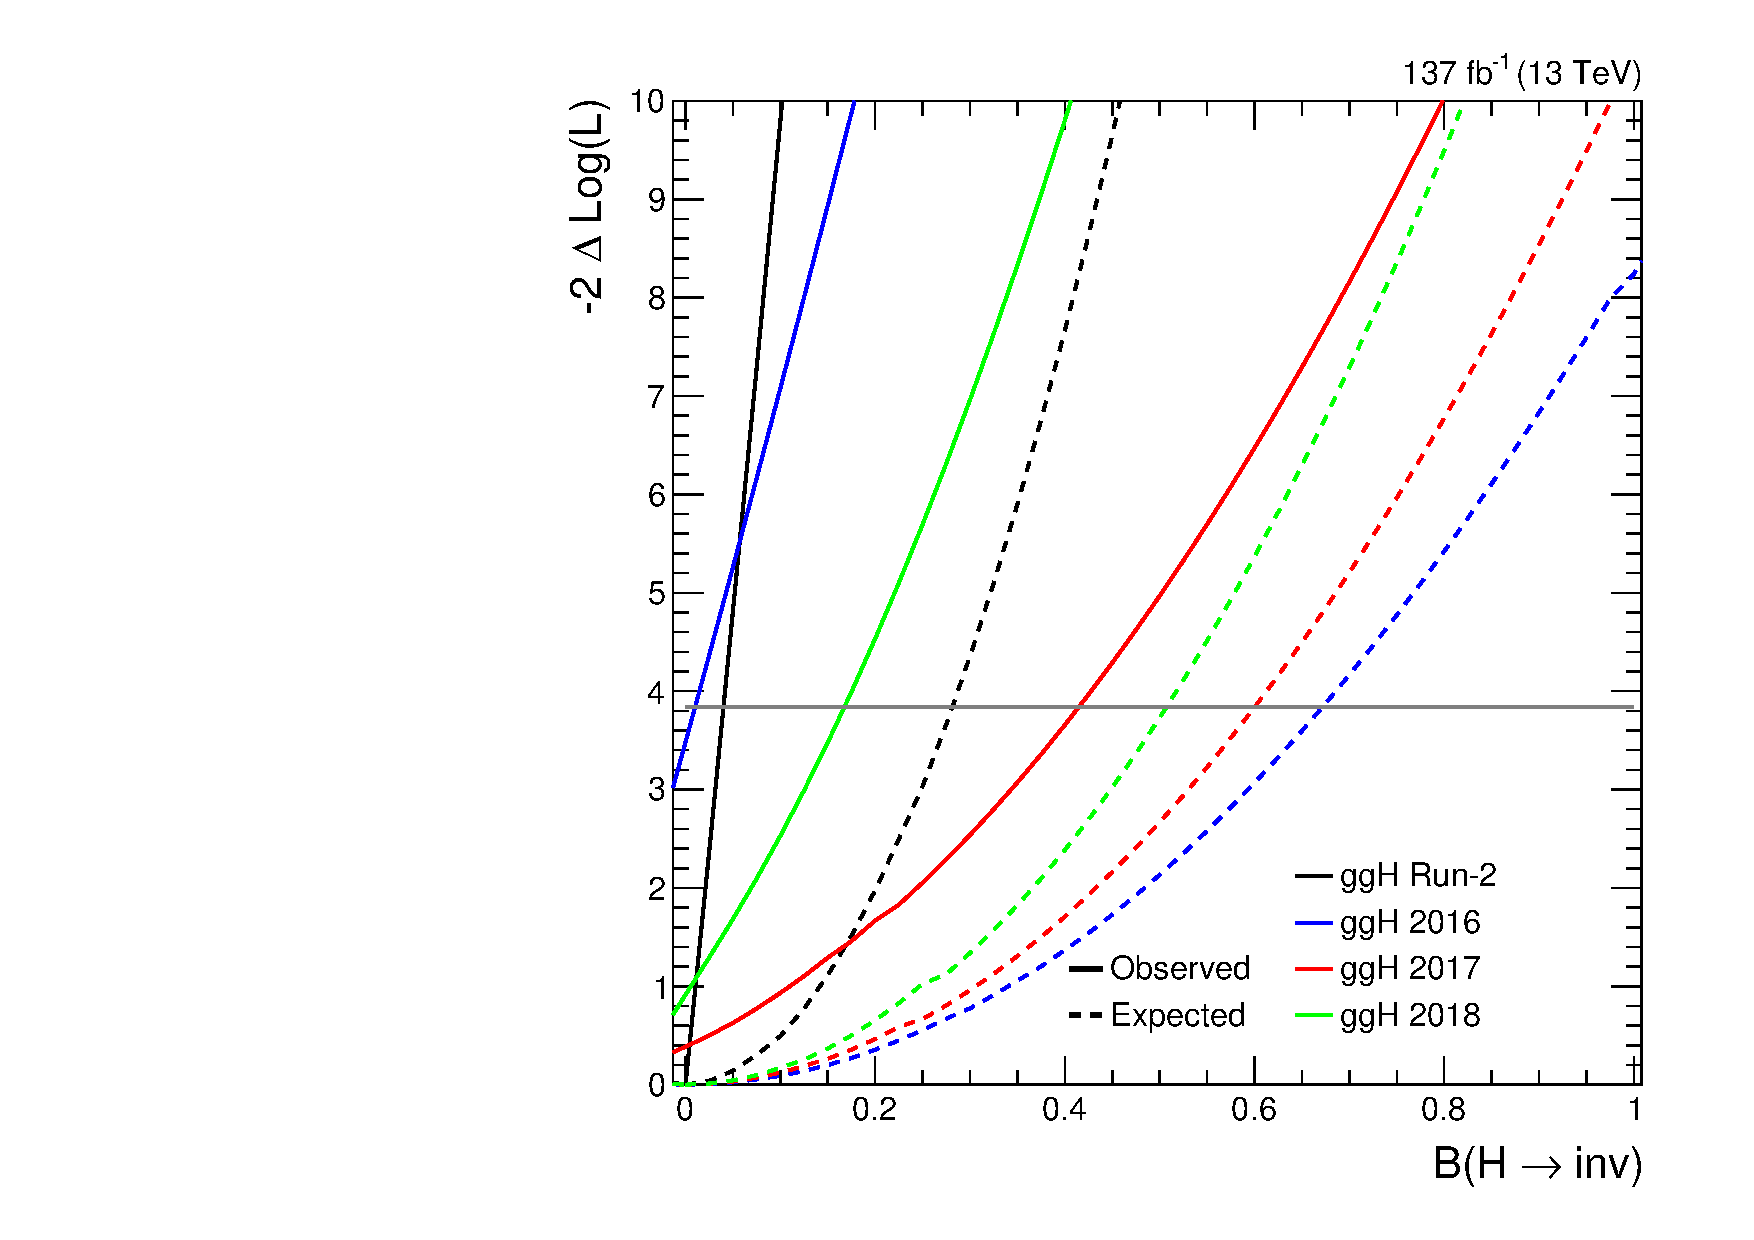
\includegraphics[width=\textwidth]{figures/likelihood_scan/profile_likelihood_scan_Run2_ggF.pdf}
        \caption{Profile likelihood --- \ggH}
    \end{subfigure}
    \caption[Observed and expected 95\,\% CL upper limit on the Higgs boson to invisible state branching fraction $\BRof{\higgstoinv}$ (left) and the corresponding profile likelihood ratio as a function of it (right) in the \ggH category]{Observed and expected 95\,\% CL upper limit on the Higgs boson to invisible state branching fraction $\BRof{\higgstoinv}$ (left) and the corresponding profile likelihood ratio as a function of it (right) in the \ggH category. The result from each data taking period is presented along with their combination.}
    \label{fig:htoinv_limit_ggF}
\end{figure}

\clearpage


%=========================================================


\section{Combined results}
\label{sec:htoinv_combined_results}

% Show the results combined over all production modes (one plot for each year), then the full combination for Run-2, ideally with VBF results as well

Upper limits for $\BRof{\higgstoinv}$ by combining all categories for the full Run-2 dataset can be shown as broken down by data taking year in Fig.~\ref{fig:htoinv_limit_likelihood_Run2_per_year} and by category in Fig.~\ref{fig:htoinv_limit_likelihood_Run2_per_cat}. Profile likelihood ratios as a function of $\BRof{\higgstoinv}$ are also presented opposite the limits. Corresponding limits and likelihood ratios for each year are displayed in Figs.~\ref{fig:htoinv_limit_likelihood_2016}, \ref{fig:htoinv_limit_likelihood_2017}, \ref{fig:htoinv_limit_likelihood_2018}, respectively, of App.~\ref{sec:limits_likelihoods_year_supplementary}.\footnote{Add some reasonable discussion of the limits and likelihoods, consistency across categories/years, once I have the final results.}\footnote{If we see worse results in 2016 compared to previous analyses, one explainer could be the signal models. It was recently discovered that signal MC used for 2016 analyses had a harder pt spectrum than what has been used in this analysis, which would give improved limits there as the distributions are shifted to higher MET and giving better signal sensitivity.}

\begin{figure}[htbp]
    \centering
    \begin{subfigure}[t]{0.45\textwidth}
        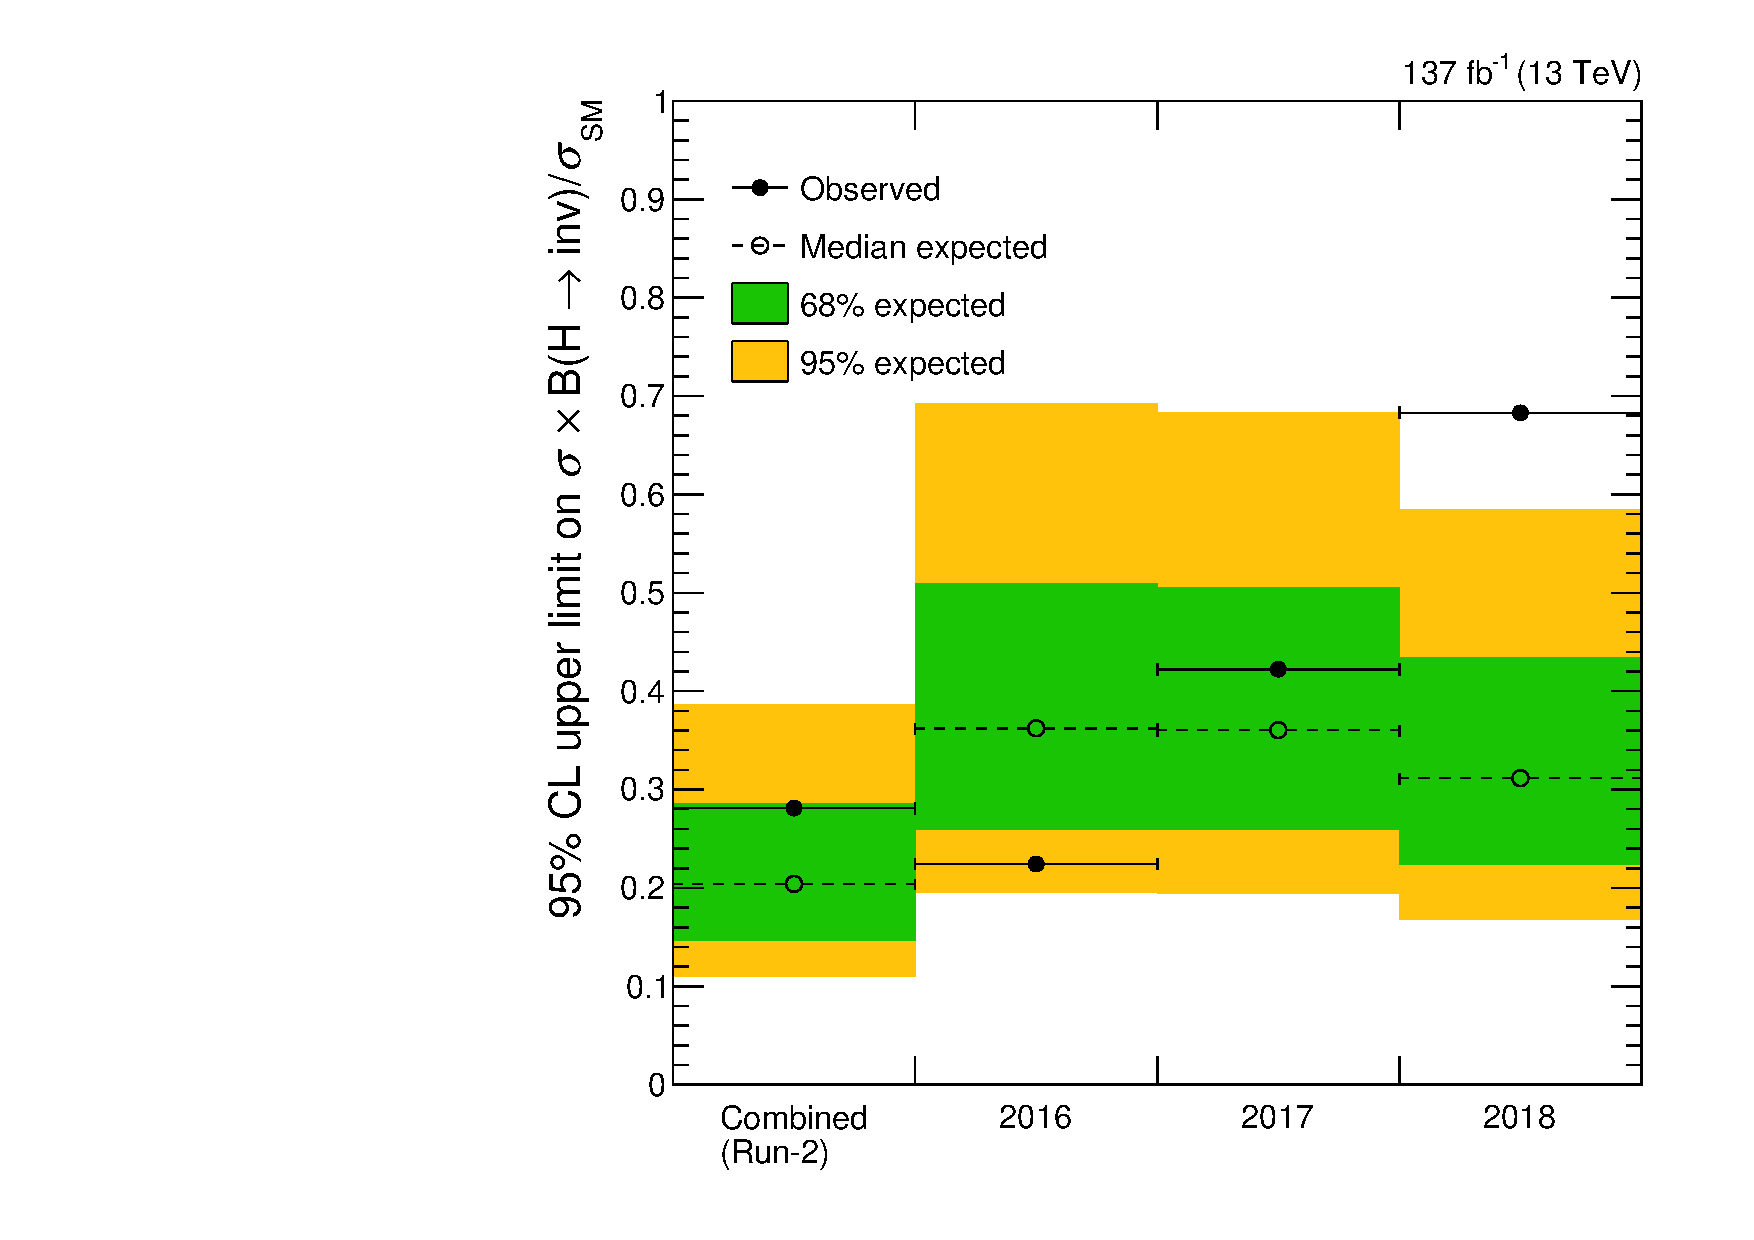
\includegraphics[width=\textwidth]{figures/limits/full_Run2/limit_Run2_comb_per_year.pdf}
        \caption{Limit --- Run-2}
    \end{subfigure}
    \hspace{0.05\textwidth}
    \begin{subfigure}[t]{0.45\textwidth}
        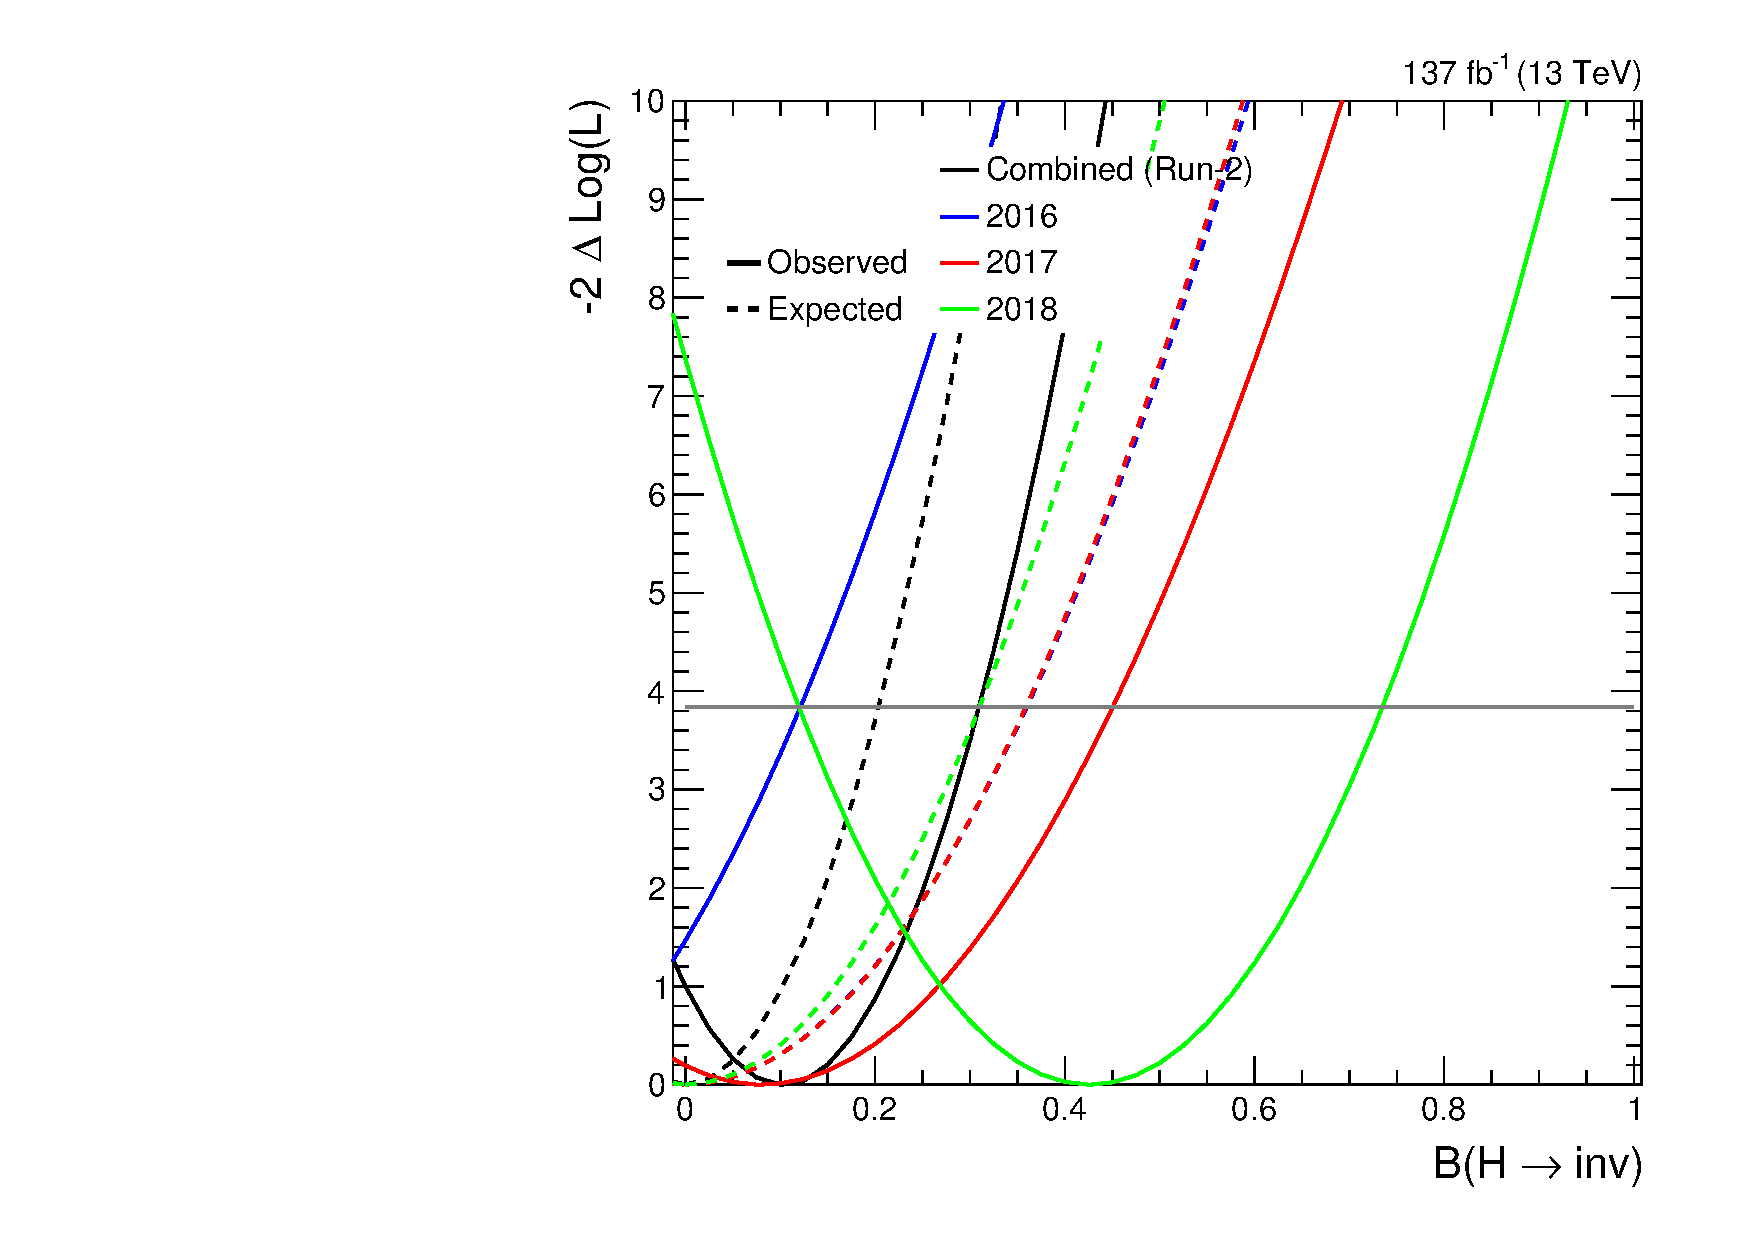
\includegraphics[width=\textwidth]{figures/likelihood_scan/profile_likelihood_scan_Run2_per_year.pdf}
        \caption{Profile likelihood --- Run-2}
    \end{subfigure}
    \caption[Observed and expected 95\,\% CL upper limit on the Higgs boson to invisible state branching fraction $\BRof{\higgstoinv}$ and the corresponding profile likelihood ratio as a function of it, for both the individual data taking years, as well as the combination of them, for the full Run-2 dataset]{Observed and expected 95\,\% CL upper limit on the Higgs boson to invisible state branching fraction $\BRof{\higgstoinv}$ (left) and the corresponding profile likelihood ratio as a function of it (right), for both the individual data taking years, as well as the combination of them, for the full Run-2 dataset. The \acrlong{sm} Higgs boson with its associated mass and production cross section are assumed.}
    \label{fig:htoinv_limit_likelihood_Run2_per_year}
\end{figure}

\begin{figure}[htbp]
    \centering
    \begin{subfigure}[b]{0.45\textwidth}  % top align since axis labels are larger for likelihood
        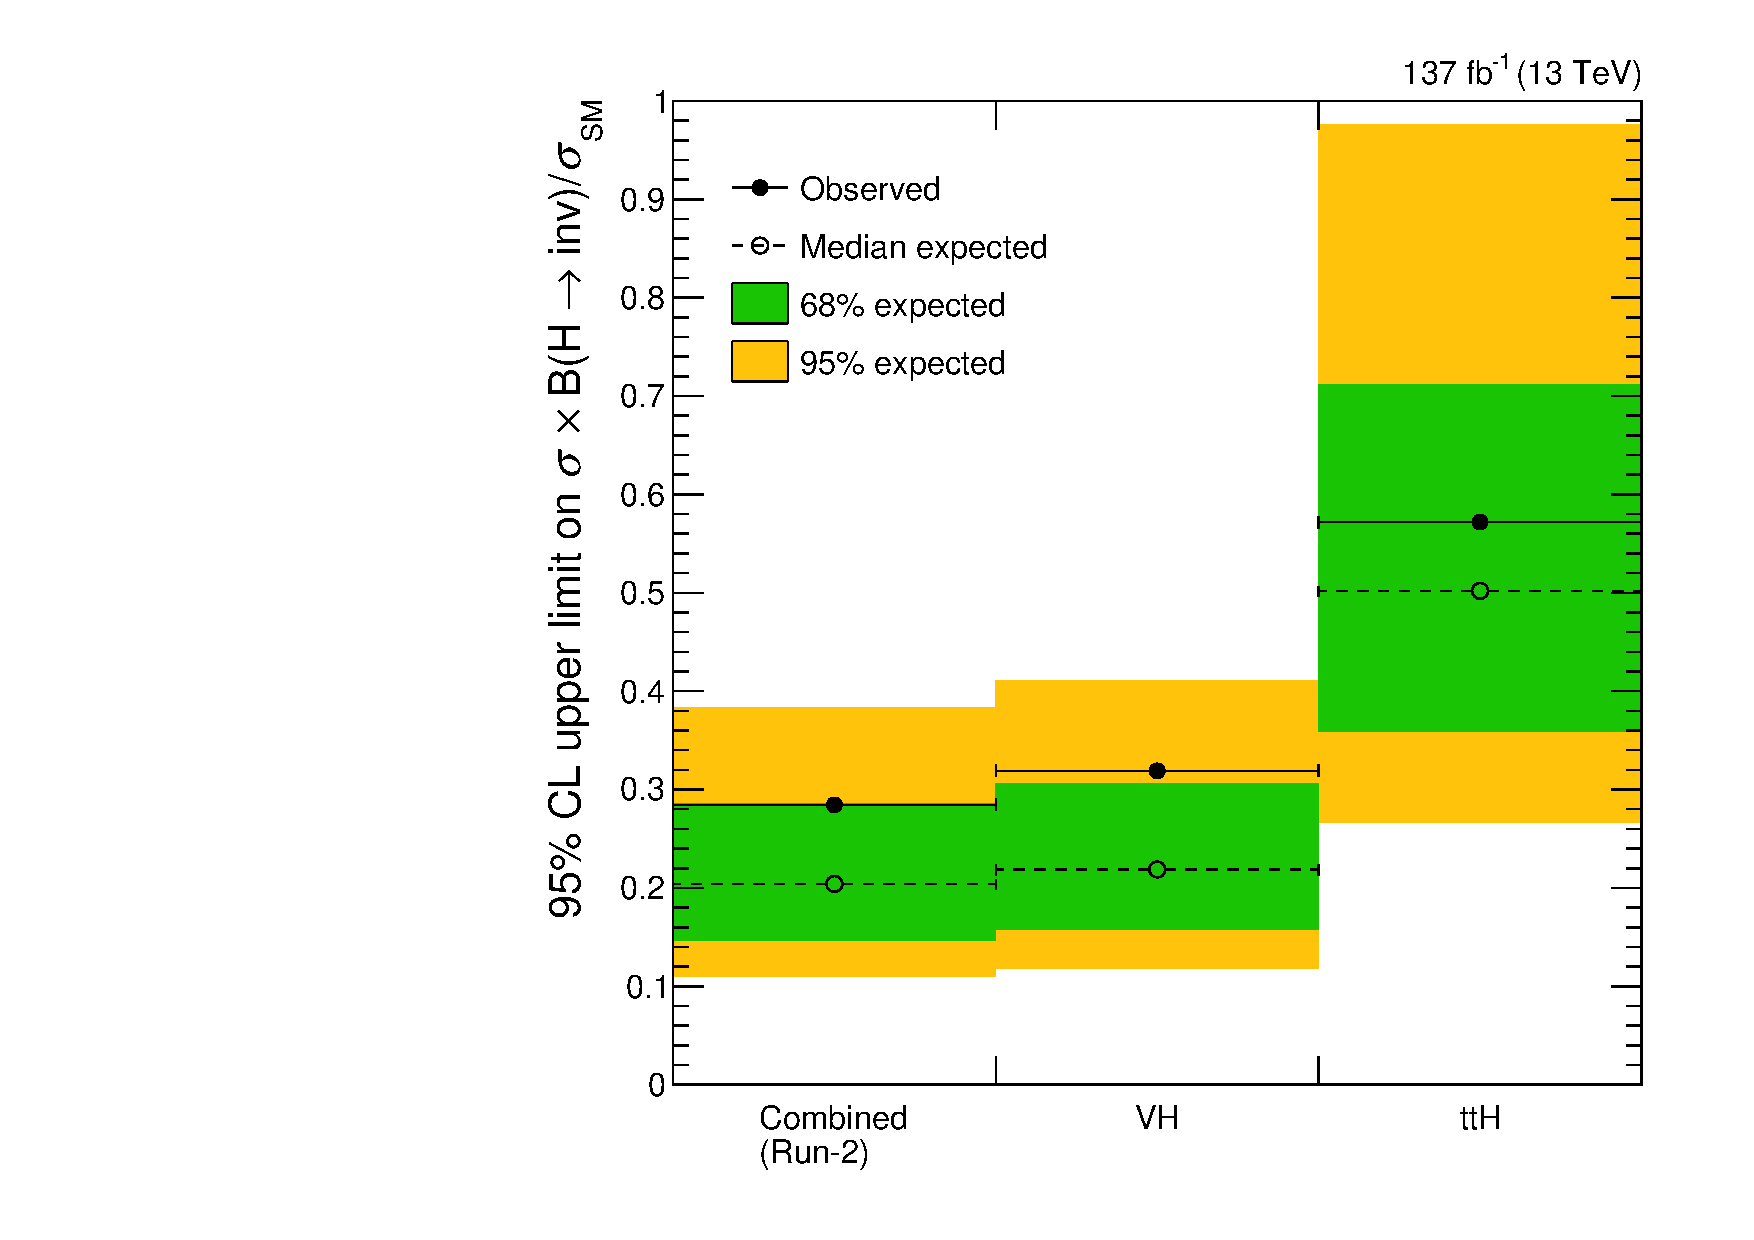
\includegraphics[width=\textwidth]{figures/limits/full_Run2/limit_Run2_comb_per_cat.pdf}
        \caption{Limit --- Run-2}
    \end{subfigure}
    \hspace{0.05\textwidth}
    \begin{subfigure}[b]{0.45\textwidth}
        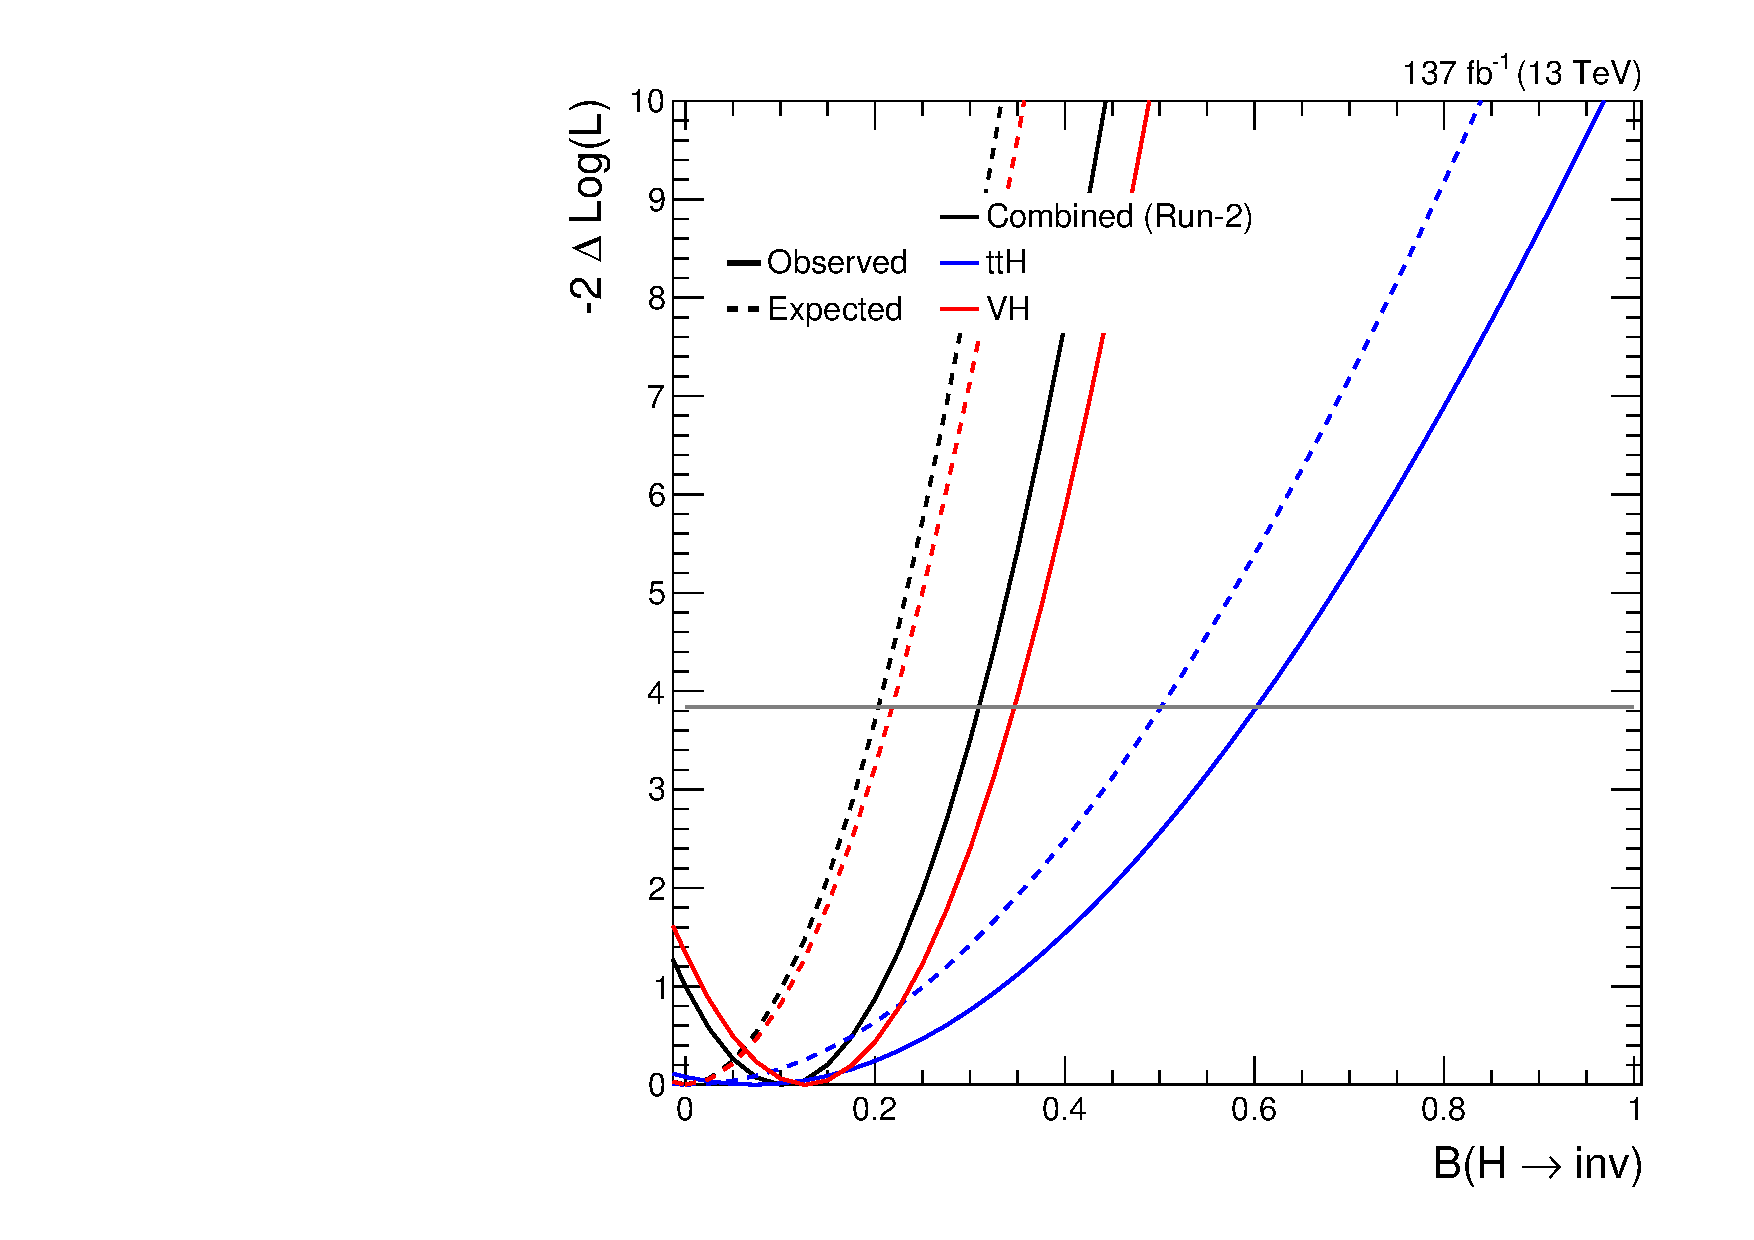
\includegraphics[width=\textwidth]{figures/likelihood_scan/profile_likelihood_scan_Run2_per_cat.pdf}
        \caption{Profile likelihood --- Run-2}
    \end{subfigure}
    \caption[Observed and expected 95\,\% CL upper limit on the Higgs boson to invisible state branching fraction $\BRof{\higgstoinv}$ and the corresponding profile likelihood ratio as a function of it, for both the individual categories, as well as the combination of them, for the full Run-2 dataset]{Observed and expected 95\,\% CL upper limit on the Higgs boson to invisible state branching fraction $\BRof{\higgstoinv}$ (left) and the corresponding profile likelihood ratio as a function of it (right), for both the individual categories, as well as the combination of them, for the full Run-2 dataset. The \acrlong{sm} Higgs boson with its associated mass and production cross section are assumed.}
    \label{fig:htoinv_limit_likelihood_Run2_per_cat}
\end{figure}

% Expected limits and likelihoods only, for Scenario 5. All limit and likelihood plots from 13th August

\begin{table}[htbp]
    \centering
    \begin{tabular}{ccccc}
        \hline\hline
        Dataset & \ttH & \VH & \ggH & Combined\\\hline
        \multirow{2}{*}{2016} & X (obs.) & X (obs.) & X (obs.) & X (obs.) \\
        & 69\,\% (exp.) & 43\,\% (exp.) & 48\,\% (exp.) & 29\,\% (exp.) \\\hline
        \multirow{2}{*}{2017} & X (obs.) & X (obs.) & X (obs.) & X (obs.) \\
        & 65\,\% (exp.) & 40\,\% (exp.) & 53\,\% (exp.) & 29\,\% (exp.) \\\hline
        \multirow{2}{*}{2018} & X (obs.) & X (obs.) & X (obs.) & X (obs.) \\
        & 62\,\% (exp.) & 36\,\% (exp.) & 34\,\% (exp.) & 23\,\% (exp.) \\\hline
        \multirow{2}{*}{Run-2} & X (obs.) & X (obs.) & X (obs.) & \textbf{X (obs.)} \\
        & 40\,\% (exp.) & 24\,\% (exp.) & 27\,\% (exp.) & \textbf{16\,\% (exp.)} \\\hline\hline
    \end{tabular}
    \caption{Observed and expected upper limits on $\BRof{\higgstoinv}$ for each category and dataset in the analysis.}
    \label{tab:hinv_limits}
\end{table}
